\documentclass[12pt]{article}

\usepackage[utf8]{inputenc}	%Encoding UTF8 per accenti
\usepackage{pdflscape} % per pagine landscape

\usepackage[T1]{fontenc}

\usepackage[italian]{babel}

\usepackage[onehalfspacing]{setspace}	%Interlinea di 1.5

\usepackage[hyperfootnotes=false]{hyperref}	%Pacchetto per coll. ipertestuali

\usepackage{tabularx}
\usepackage{longtable,array} %Per Tabelle potenzialmente multipagina
\usepackage{fancyhdr}  % per gli header e footer
\usepackage{graphicx}  %per le immagini
\usepackage{flafter}
\usepackage{listings} %per i listati di codice
\usepackage[font=small,labelfont=bf]{caption}

\usepackage{framed}

\usepackage[headheight=2cm, headsep=0.5cm, a4paper, margin=3cm]{geometry}
\usepackage[bottom]{footmisc}

\hypersetup{colorlinks=true}		%Configurazione colore link documento
\hypersetup{linkcolor= blue}
\renewcommand\UrlFont{\color{blue}\rmfamily\itshape} %Forzato colore blu su tutti i link ESTERNI

\usepackage[dvipsnames,table]{xcolor}
\definecolor{bluelogo}{HTML}{415A66}
\definecolor{grigio}{HTML}{D0D0D0}
\usepackage{makecell}

\renewcommand{\footrulewidth}{0.1pt}
\newcommand{\glossario}{\textsubscript{G} }

\usepackage{fancyhdr}
\usepackage{lastpage}
 
\pagestyle{fancy}

\fancyhf{}

\lhead{
\includegraphics[scale=0.08]{./images/logo.png}}
\rhead{\rightmark}

\lfoot{Piano di Progetto v2.0.0}
\cfoot{}
\rfoot{Pagina \thepage \hspace{1pt} di \pageref*{LastPage}}

\makeindex
\setcounter{secnumdepth}{4}
\setcounter{tocdepth}{4}

%\lhead{
\includegraphics[scale=0.08]{./images/logo.png}}
%\usepackage[headheight=2cm, headsep=0.5cm, a4paper, margin=3cm]{geometry}

\newcolumntype{C}[1]{>{\centering\arraybackslash}m{#1}}
\usepackage{eurosym}

\usepackage{grffile}
\usepackage{float}




\usepackage{graphicx}

% Ridefinizione dei nomi degli indici
\renewcommand{\listtablename}{Indice delle Tabelle}
\renewcommand{\listfigurename}{Indice di Figure e Grafici}


\begin{document}
\begin{titlepage}
\thispagestyle{empty}
\pagenumbering{gobble}

\begin{center}

\includegraphics[scale=0.3]{./images/logo.png}\\
\large \textbf{Agents of S.W.E. - Progetto "G\&B"}
\vfill
\Huge \textbf{Piano di Progetto}
\vfill
\large
\renewcommand{\arraystretch}{1.3}
\begin{tabular}{r|l}


\textbf{Versione} & 2.0.0\\
\textbf{Approvazione} & Diego Mazzalovo\\
\textbf{Redazione} & \parbox[t]{5cm}{Carlotta Segna\\Diego Mazzalovo\\Matteo Slanzi\\Luca Violato}\\
\textbf{Verifica} & \parbox[t]{5cm}{Marco Chilese \\ Marco Favaro\\Luca Violato}\\
\textbf{Stato} & Approvato\\
\textbf{Uso} & Esterno\\
\textbf{Destinato a} & \parbox[t]{5cm}{Agents of S.W.E. \\Prof. Tullio Vardanega\\Prof. Riccardo Cardin \\ Zucchetti S.p.A.}
\end{tabular}
\vfill
\small
\texttt{agentsofswe@gmail.com}
\end{center}
\end{titlepage}

\pagebreak

\pagenumbering{arabic}

\section{Changelog}

\begin{center}
\begin{longtable}[c]{|m{.11\textwidth}|m{.13\textwidth}|m{.1\textwidth}|m{.19\textwidth}|p{.33\textwidth}|}
\hline
\rowcolor{bluelogo}\textbf{\textcolor{white}{Versione}} & \textbf{\textcolor{white}{Data}} & \textbf{\textcolor{white}{Autore}} & \textbf{\textcolor{white}{Ruolo}} & \textbf{\textcolor{white}{Descrizione}}\\
\hline \hline
\endfirsthead
0.0.1 & 2018-11-23 & Luca Violato & Amministratore & Strutturazione del Documento \\
\hline
\rowcolor{grigio} 0.0.2 & 2018-12-18 & Carlotta Segna & Responsabile & Standardizzazione tabella \\
\hline
\caption{Changelog del documento}
\end{longtable}
\end{center}
\newpage

\tableofcontents

% Inclusione degli indici di tabelle e immagini
\listoftables
\listoffigures
%\pagenumbering{arabic}

\pagebreak

\section{Introduzione}\label{Intro}

\subsection{Scopo del Documento}
Il presente documento è stato realizzato con lo scopo di presentare le funzionalità del prodotto e spiegare, in modo intuitivo ma preciso, le modalità di utilizzo del plug-in \textit{G\&B}.

\subsection{Scopo del Prodotto}\label{ScopoProdotto}
Lo scopo del prodotto è la creazione di un plug-in per la piattaforma open source di visualizzazione e gestione dati, denominata \textit{Grafana}\glossario, con l'obiettivo di creare un sistema di alert\glossario dinamico per monitorare la "liveliness\glossario" del sistema a supporto dei processi DevOps\glossario e per consigliare interventi nel sistema di produzione del software. In particolare, il plug-in utilizzerà dati in input forniti ad intervalli regolari o con continuità, ad una rete bayesiana\glossario per stimare la probabilità di alcuni eventi, segnalandone quindi il rischio in modo dinamico, prevenendo situazioni di stallo.



\pagebreak

\section{Analisi dei Rischi}
\label{RischiIntroduzione}

L'analisi dei rischi prevede la valutazione preventiva dei possibili problemi che possono verificarsi durante lo svolgimento del progetto. \\
I rischi sono catalogati in base a tipologie stabilite a priori all'interno del gruppo. 
Ogni rischio sarà inserito in una particolare categoria:
\begin{itemize}
\item Rischi relativi ai Componenti del Gruppo \texttt{Agents of S.W.E.} (G);
\item Rischi relativi alle Tecnologie da utilizzare(T);
\item Rischi relativi alla Gestione del Lavoro(L);
\item Rischi relativi ai Requisiti\glossario Richiesti(R).  
\end{itemize}

L'utilizzo dei numeri è incrementale e la suddivisione dei rischi in sottocategorie non interferisce con l'incremento numerico, in modo tale da avere una visione complessiva del numero di possibili rischi che possono intercorrere durante lo svolgimento del progetto. \\

\subsection{Identificazione}
\label{RischiIdentificazione}

\begin{longtable}{|C{.13\textwidth}|C{.36\textwidth}|C{.22\textwidth}|C{.17\textwidth}|}
\hline
\rowcolor{bluelogo}\textbf{\textcolor{white}{Rischio}} & \textbf{\textcolor{white}{Descrizione}} & \textbf{\textcolor{white}{Rilevamento}} & \textbf{\textcolor{white}{Grado di rischio}}\\
\hline \hline
\endhead
G01 &  Alcuni componenti del gruppo non si conoscono tra di loro. Questo potrebbe causare problematiche relative alla comunicazione intragruppo. & Il \textit{Responsabile} avrà il compito di controllare e risolvere eventuali diatribe che  potrebbero venire a crearsi. & Occorrenza:  \textbf{Media}  Pericolosità:  \textbf{Media} \\
\hline
\rowcolor{grigio} \textbf{Piano di Contingenza} & \multicolumn{3}{ l |}{\parbox[c][2cm]{12cm}{La rotazione dei compiti avverrà in modo tale da far conoscere tutte le componenti del gruppo tra di loro, per trovare il corretto equilibrio in termini di efficienza ed efficacia.}} \\

\hline
G02 &  Alcuni membri del gruppo hanno impegni lavorativi e questo comporterà una presenza minore durante lo svolgimento delle componenti progettistiche.  & I vari membri del gruppo hanno impegni diversi. Fissare un appuntamento comune può essere un problema. &  Occorrenza:  \textbf{Bassa}  Pericolosità:  \textbf{Alta} \\
\hline
\rowcolor{grigio} \textbf{Piano di Contingenza} & \multicolumn{3}{ l |}{\parbox[c][2cm]{12.0cm}{La creazione di un calendario comune per il gruppo permette di accordarsi in modo comune e più semplice.}}\\

\hline	
G03 &  Quasi nessuno dei membri del gruppo ha avuto precedenti esperienze lavorative in team. Questo potrebbe implicare problemi nello svolgimento delle attività e conseguenti ritardi.  & Mancato rispetto delle milestone\glossario prestabilite. &  Occorrenza:  \textbf{Alta}  Pericolosità:  \textbf{Alta} \\
\hline
\rowcolor{grigio} \textbf{Piano di Contingenza} & \multicolumn{3}{ l |}{\parbox[c][2cm]{12.0cm}{Analisi della milestone non rispettata, al fine di migliorare la gestione del tempo per le milestone successive.}}\\

\hline		
T04 &  Certe tecnologie da usare sono sconosciute a tutti i membri del gruppo, mentre altre solo a certi membri. Ciò potrebbe causare ritardi nell'avanzamento del progetto. & Sarà responsabilità di ogni membro del gruppo comunicare al \textit{Responsabile} le conoscenze mancanti sulle tecnologie da utilizzare. &  Occorrenza:  \textbf{Media}  Pericolosità:  \textbf{Alta} \\
\hline
\rowcolor{grigio} \textbf{Piano di Contingenza} & \multicolumn{3}{ l |}{\parbox[c][3cm]{12.0cm}{Coloro che conoscono determinate tecnologie sconosciute ad altri, dovranno aiutare chi non le conosce. Per quelle sconosciute a tutti, lo studio verrà suddiviso in maniera equa e successivamente ogni membro condividerà ciò che ha appreso con gli altri.}} \\

\hline		
T05 &  L'utilizzo da parte del gruppo di strumentazione software di terzi per la gestione del progetto, comporta che, in caso di malfunzionamenti, potrebbero verificarsi ritardi o eventuali perdite di dati.  & Il problema non sarà facilmente riscontrabile, in quanto dipende da fattori esterni ed eventuali guasti non sono identificabili prima che si verifichino. &  Occorrenza:  \textbf{Bassa}  Pericolosità:  \textbf{Alta} \\
\hline
\rowcolor{grigio} \textbf{Piano di Contingenza} & \multicolumn{3}{ l |}{\parbox[c][3cm]{12.0cm}{Per far fronte ad eventuali malfunzionamenti di \textit{Github}\glossario et similia, ogni membro del gruppo provvederà ad effettuare dei backup ad intervalli regolari dei dati, in modo da poterli recuperare in caso di bisogno.}}\\

\hline		
T06 & I PC dei singoli membri del gruppo potrebbero guastarsi ed eventuali malfunzionamenti hardware potrebbero causare la perdita di dati, oltre a possibili ritardi nel ripristinare lo stato ottimale dei mezzi di lavoro.  & In caso di problemi, l'interessato provvederà ad avvisare gli altri componenti del gruppo. &   Occorrenza:  \textbf{Bassa}  Pericolosità:  \textbf{Media} \\
\hline
\rowcolor{grigio} \textbf{Piano di Contingenza} & \multicolumn{3}{ l |}{\parbox[c][3cm]{12.0cm}{Ogni membro del gruppo effettuerà dei backup settimanali dei dati, in modo da poter recuperare la maggior parte del lavoro in caso di guasti.}}\\

\hline
T07 & L'utilizzo di software cross-platform\glossario/open-source\glossario può causare problemi di porting a seconda del 
sistema operativo, portando al malfunzionamento o al non utilizzo di tale software. & I membri forniranno all'\textit{Amministratore} il sistema operativo in uso, in modo da prevedere il malfunzionamento di alcuni software su piattaforme differenti. &  Occorrenza:  \textbf{Bassa}  Pericolosità:  \textbf{Bassa} \\
\hline
\rowcolor{grigio} \textbf{Piano di Contingenza} & \multicolumn{3}{ l |}{\parbox[c][2cm]{12.0cm}{Prima dell'effettivo inizio del progetto, l'\textit{Amministratore} provvederà a ricercare software disponibili in ognuno di questi sistemi.}}\\

\hline		
T08 & Per l'apprendimento di certe tecnologie sconosciute al gruppo, potrebbe essere richiesto più tempo rispetto a quello programmato.  & Sarà compito del \textit{Responsabile} valutare la complessità di tali tecnologie. &  Occorrenza:  \textbf{Media}  Pericolosità:  \textbf{Media} \\
\hline
\rowcolor{grigio}\textbf{Piano di Contingenza} & \multicolumn{3}{ l |}{\parbox[c][3cm]{12.0cm}{Per far fronte a ciò, qualora sia possibile, saranno richiesti incontri con la proponente per la spiegazione di eventuali tecnologie di difficile apprendimento.}}\\

\hline
L09 & Nessun membro del gruppo ha precedenti esperienze nella pianificazione delle attività. & Il \textit{Responsabile} terrà traccia degli effettivi tempi di sviluppo. &   Occorrenza:  \textbf{Alta}  Pericolosità:  \textbf{Alta} \\
\hline
\rowcolor{grigio} \textbf{Piano di Contingenza} & \multicolumn{3}{ l |}{\parbox[c][4cm]{12.0cm}{Verranno stabilite delle milestones, in modo che ad ognuna di esse possa essere valutato l'adempimento o meno dei compiti prestabiliti. In caso negativo, il lavoro arretrato verrà ridistribuito tra i membri del gruppo. Inoltre, sarà possibile ripianificare le attività fino alla prossima milestone con maggior precisione.}} \\

\hline
L10 & La pianificazione prevede un costo per le attività. Tutti i membri del gruppo sono alla prima esperienza su un progetto simile, questo potrebbe portare a delle valutazioni errate sui costi complessivi del progetto. & In caso di ritardo nello svolgimento delle attività, il/i diretto/i interessato/i  lo comunicherà/nno al \textit{Responsabile}.  &  Occorrenza:  \textbf{Media}  Pericolosità:  \textbf{Media} \\
\hline
\rowcolor{grigio} \textbf{Piano di Contingenza} & \multicolumn{3}{ l |}{\parbox[c][3cm]{12.0cm}{Il \textit{Responsabile} valuterà di volta in volta le attività in modo tale da far quadrare i costi prestabiliti nel preventivo.}}\\

\hline
R11 & Potrebbero essere rivalutati i requisiti da parte della proponente \textit{Zucchetti S.p.A.} o da parte del gruppo in caso di necessità. Ciò richiederebbe una revisione parziale oppure completa dell'Analisi dei requisiti, portando così ritardi nelle consegne. & Già dalle prime fasi, il gruppo cercherà di comunicare il più possibile con la proponente, in modo da far emergere ogni possibile necessità nella modifica dei requisiti. &  Occorrenza:  \textbf{Bassa}  Pericolosità:  \textbf{Alta} \\
\hline
\rowcolor{grigio} \textbf{Piano di Contingenza} & \multicolumn{3}{ l |}{\parbox[c][3cm]{12.0cm}{Il gruppo cercherà di discutere apertamente con la proponente le modifiche sui requisiti, cercando di trovare un punto comune che soddisfi entrambe le parti.}} \\

\hline
R12 & L'analisi del capitolato scelto e la valutazione dei suoi requisiti possono essere fraintesi, questo può creare delle divergenze tra le aspettative della proponente e la visione del gruppo sul progetto. & Durante l'attività di Analisi dei requisiti, verranno effettuati degli incontri con la proponente per ridurre al minimo possibili incomprensioni ed errori. &  Occorrenza:  \textbf{Bassa}  Pericolosità:  \textbf{Bassa} \\
\hline
\rowcolor{grigio} \textbf{Piano di Contingenza} & \multicolumn{3}{ l |}{\parbox[c][4cm]{12.0cm}{Il gruppo esporrà negli incontri con la proponente, eventuali dubbi in modo da chiarire ogni requisito richiesto per il corretto sviluppo del progetto. Possibili errori dovranno essere corretti in seguito all'esito di ogni revisione.}}\\
\hline

\caption{Identificazione dei Rischi}
\label{Tabella Identificazione dei Rischi}
\end{longtable}

\pagebreak

\section{Modello di Sviluppo}

Dopo un'attenta analisi dei vari modelli di sviluppo il gruppo \texttt{Agents of S.W.E.} ha scelto di utilizzare il modello di tipo \textbf{incrementale}.

\subsection{Modello Incrementale}

\begin{figure}[h]
	\centering
  		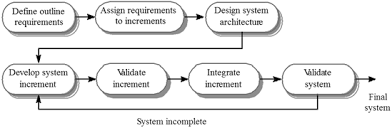
\includegraphics[width=0.7\linewidth]{./images/modelloincrementale.png}
  		\caption{Modello Incrementale.}
  		\label{fig:Modello Incrementale}
\end{figure}

Il modello incrementale prevedere rilasci multipli e successivi del prodotto ed ogni rilascio prevede un incremento delle sue funzionalità. \\
Con questo modello vengono pianificati quanti incrementi verranno effettuati basandosi sui requisiti\glossario obbligatori ed opzionali richiesti dalla proponente, aggiungendovi delle priorità di sviluppo in modo tale che elementi con priorità maggiore vengano sviluppati prima di elementi con priorità minore.\\
Il prodotto finale non sarà rilasciato nella sua completezza in un solo momento ma prevederà, appunto, degli incrementi. \\
E' fondamentale decidere i requisiti con completezza prima di iniziare lo sviluppo dell'attuale incremento, mentre requisiti aggiuntivi per incrementi futuri sono adeguati. Per ogni sviluppo delle parti è necessario analizzare il suo grado di efficacia prima di integrare le parti tra di loro. Terminato l'incremento attuale si andrà avanti con l'incremento successivo scelto precedentemente, qualora il prodotto non sia completo. \\
Il \textbf{vantaggio} di utilizzare questo modello racchiude, tra le varie, un rilascio delle funzionalità base nei primi incrementi, il che comporta una maggiore verifica e quindi una maggiore stabilità. Oltretutto i primi incrementi possono derivare da una prototipazione, la quale aiuta a fissare meglio i requisiti per gli elementi successivi. Un ulteriore vantaggio è la riduzione del rischio di fallimento, senza azzerarlo in quanto costi aggiuntivi posso derivare dalla caduta nell'iterazione\glossario.


\pagebreak

\section{Pianificazione}

Basandosi sulle scadenze esposte nel capitolo §1.5 si è deciso di sviluppare il progetto suddividendolo sulla base dello standard ISO/IEC 12207:1995, che prevede le seguenti fasi:
\begin{itemize}
	\item Attività preliminari di avvio ed analisi dei requisiti;
	\item Progettazione architetturale;
	\item Progettazione di dettaglio e codifica;
	\item Validazione e collaudo.
\end{itemize}

\begin{longtable}{ m{8cm} m{3cm} p{3cm} }
\hline

\rowcolor{bluelogo}\color{white}\textbf{Fase} & \color{white}\textbf{Inizio} & \color{white}\textbf{Fine} \\
\hline
\rowcolor{beigechiaro} \color{black} Avvio ed analisi requisiti & 15/11/2018 & 14/01/2019 \\
\rowcolor{beigescuro} \color{black} Risanamento criticità & 22/01/2019 & 28/01/2019 \\
\rowcolor{beigechiaro} \color{black} Progettazione architetturale & 29/01/2019 & 08/03/2019 \\
\rowcolor{beigescuro} \color{black} Risanamento criticità & 16/03/2019 & 19/03/2019 \\
\rowcolor{beigechiaro} \color{black} Progettazione di dettaglio e codifica & 20/03/2019 & 12/04/2019 \\
\rowcolor{beigescuro} \color{black} Validazione e collaudo & 20/04/2019 & 10/05/2019 \\

\hline
\end{longtable}

La prima fase sarà a carico del gruppo \texttt{Agents of S.W.E.} mentre le ulteriori tre fasi saranno a carico del committente. \\
Nonostante la scelta di adottare lo standard ISO/IEC, abbiamo deciso di aggiungere un incremento tra le prime due fasi che consiste in un periodo di sanazione delle criticità trovate dopo un'attenta analisi della documentazione, che avviene non solo da parte del gruppo \texttt{Agents of S.W.E.}, ma anche da parte della proponente. 

\subsection{Attività preliminari di avvio ed analisi dei requisiti}

Il periodo di analisi va dal 15/11/2018, data di formazione dei gruppi, e termina il 14/01/2019 con la consegna della documentazione relativa alla RR.

\subsubsection{Incrementi}

Il primo periodo prevede 6 incrementi e le principali operazioni svolte sono: 
\begin{itemize}
	\item \textbf{Analisi dei Requisiti}: all'interno del documento \textit{Analisi dei Requisiti} vengono inseriti tutti i requisiti individuati dagli Analisti, analizzando il capitolato d'appalto. Questa risulta essere un'attività particolarmente importante poiché l'errata analisi comporterebbe un impedimento nell'avanzamento del progetto.
	\item \textbf{Glossario}: il documento \textit{Glossario} racchiuderà tutti i termini ambigui o poco chiari che vengono individuati durante la redazione dei documenti;
	\item \textbf{Lettera di Presentazione}: l'attività prevede la stesura della \textit{Lettera di Presentazione} dichiarando il gruppo \texttt{Agents of S.W.E.} come fornitore;
	\item \textbf{Norme di Progetto}: tutte le norme che vengono stabilite saranno inserite all'interno del documento \textit{Norme di progetto} individuate dall'Amministratore. Ha lo scopo di uniformare le modalità di lavoro che dovranno essere attuate da tutti i membri del gruppo. Consiste in un'attività critica in quanto fondamentali per la stesura della documentazione;
	\item \textbf{Piano di Progetto}: è compito del Responsabile analizzare attività e scadenze al fine di ottenere una buona riuscita del progetto ed è compito dell'Amministratore analizzare i rischi nei quali si può incorrere. Le attività e le risorse vengono suddivise per l'intera durata del progetto ed inserite all'interno del documento \textit{Piano di Progetto}, necessario e vincolante per la stesura della \textit{Lettera di presentazione};
	\item \textbf{Piano di Qualifica}: i Progettisti avranno il compito di cercare un elenco di attività e metodi utili al fine di garantire una buona qualità di prodotto. Questi verranno racchiusi all'interno del documento \textit{Piano di Qualifica};
	\item \textbf{Studio di fattibilità}: consiste nell'analisi preliminare dei vari capitolati proposti ed è essenziale alla fine della scelta del capitolato da svolgere. L'analisi verrà inserita all'interno del documento \textit{Studio di fattibilità}; questa risulta essere un'attività bloccante per l'inizio dell'attività di Analisi dei Requisiti.  
\end{itemize}

\subsection{Risanamento criticità}

Con \textit{Risanamento delle criticità}, fase all'infuori dello standard ISO, intendiamo una periodo da noi programmato in cui andremo ad analizzare le varie criticità che sono emerse alla fine del primo incremento, dopo la sua analisi sia da parte della proponente che da parte del gruppo. \\
La scelta di inserire questo tra la prima e la seconda fase è guidata dal fatto che per procedere è necessario aver risolto tutti i problemi riscontrati nelle produzioni precedenti, in particolar modo la seconda fase, individuata dallo standard, prevede la \textit{Progettazione architetturale} ed è quindi fondamentale sanare i problemi sorti nel primo periodo. 

\subsection{Progettazione architetturale}

Il periodo di \textit{Progettazione architetturale} inizia dalla fine del periodo di \textit{Risanamento criticità} e termina con la consegna del nuovo incremento (quindi dal 29/01/2018 al 08/03/2018), il quale prevede le operazioni riportate nella sottosezione seguente.

\subsubsection{Incrementi}
\begin{itemize}
	\item \textbf{Incremento e verifica}: all'inizio del periodo vengono svolte attività di incremento e verifica su vari documenti (\textit{Norme di progetto, Piano di progetto, Piano di qualifica});
	\item \textbf{Studio tecnologie}: prevede un continuo approfondimento delle tecnologie necessarie allo svolgimento del progetto; 
	\item \textbf{Technology Baseline}\glossario: questa attività prevede l'analisi e la scelta di tecnologie, framework\glossario e librerie\glossario da utilizzare. In questa fase, inoltre, è previsto lo sviluppo del \textit{Proof of concept}\glossario;
	\item \textbf{Glossario}: aggiunta e modifica dei termini in itinere;  
	\item \textbf{Verifica}: cinque giorni prima della fine del periodo sarà compito dei Verificatori analizzare i risultati della seconda fase segnalando, a chi di dovere, gli errori o le imprecisioni riscontrate.
\end{itemize}

\subsection{Risanamento criticità}
Con \textit{Risanamento delle criticità}, fase all'infuori dello standard ISO, intendiamo una periodo da noi programmato in cui andremo ad analizzare le varie criticità che sono emerse alla fine del primo incremento, dopo la sua analisi sia da parte della proponente che da parte del gruppo. \\

\subsection{Progettazione di dettaglio e codifica}
Il periodo di \textit{Progettazione di dettaglio e codifica} va dal giorno dopo la fine del periodo di \textit{Risanamento delle criticità}, cioè il 20/03/2019, e termina con la consegna dei documenti per la RQ, cioè il 12/04/2019.\\

\subsubsection{Incrementi}
Gli incrementi che si andranno ad attuare durante questo periodo sono:
\begin{itemize}
	\item \textbf{Incremento e verifica}: \item \textbf{Incremento e verifica}: all'inizio del periodo vengono svolte attività di incremento e verifica su vari documenti (\textit{Norme di progetto, Piano di progetto, Piano di qualifica e Technology Baseline});
	\item \textbf{Glossario}: prevede l'aggiunta di nuovi termini al \textit{Glossario} ed il suo miglioramento;
	\item \textbf{Product Baseline}\glossario: presenta la baseline\glossario architetturale del prodotto, coerente rispetto a quando riportato nella \textit{Technoly Baseline}. Al suo interno contiene i diagrammi delle classi e di sequenza, la contestualizzazione dei design pattern adottati nell'architettura del prodotto. 
	\item \textbf{Codifica}: prevede la scrittura del codice e relativa verifica\glossario di esso;
	\item \textbf{Manuale utente}: consiste nella redazione del \textit{Manuale utente}, contente le indicazioni d'utilizzo del prodotto;
	\item \textbf{Lettera di Presentazione}: prevede la stesura della \textit{Lettera di presentazione} per la partecipazione alla RQ.
\end{itemize}

\subsection{Validazione e collaudo}
Il periodi di \textit{Validazione e collaudo} inizia il 20/04/2018 e termina il 10/05/2018 con la consegna dei documenti per la RA. 

\subsubsection{Incrementi}
Durante questo periodo saranno svolti i seguenti incrementi:
\begin{itemize}
	\item \textbf{Incremento e Verifica}: \item \textbf{Incremento e verifica}: all'inizio del periodo vengono svolte attività di incremento e verifica su vari documenti (\textit{Norme di progetto, Piano di progetto, Piano di qualifica e Technology Baseline});
	\item \textbf{Glossario}: prevede l'aggiunta di nuovi termini al \textit{Glossario} ed il suo miglioramento;
	\item \textbf{Validazione e collaudo}: prevede lo sviluppo ultimo del prodotto, inserendovi miglioramenti e svolgendo ulteriori test al fine di assicurare e completare il completo soddisfacimento dei requisiti;
	\item \textbf{Manuale utente}: prevede il miglioramento e completamento del \textit{Manuale utente}, contente le indicazioni di utilizzo del prodotto.
\end{itemize}




\pagebreak

\section{Preventivo}

La sezione Preventivo ha lo scopo di stimare il costo complessivo per la prestazione elargita. \\ 
La suddivisione oraria segue alcune regole comuni per ogni membro:
\begin{itemize}
	\item I componenti dovranno svolgere tutti i ruoli almeno una volta;
	\item Ogni componente dovrà lavorare almeno 8 ore per ogni ruolo;
	\item Tutti i componenti avranno lo stesso numero ore di lavoro ad ogni revisione.
\end{itemize}
Le sigle per i vari ruoli sono:
\begin{itemize}
	\item RE: Responsabile;
	\item AM: Amministratore;
	\item AN: Analista;
	\item PJ: Progettista;
	\item PR: Programmatore;
	\item VE: Verificatore.
\end{itemize}

\newpage
\subsection{Avvio ed Analisi dei Requisiti}
\subsubsection{Prospetto orario}

Nel periodo di \textit{Avvio ed Analisi dei Requisiti} la suddivisione oraria, per ogni membro del gruppo, è la seguente:

\begin{longtable}{|C{.30\textwidth}|C{.06\textwidth}|C{.06\textwidth}|C{.06\textwidth} | C{.06\textwidth}| C{.06\textwidth} | C{.06\textwidth} | C{.10\textwidth} |}
\hline
\textbf{Nome} & \textbf{RE} & \textbf{AM} & \textbf{AN} & \textbf{PJ} & \textbf{PR} & \textbf{VE} & \textbf{Totale}\\
\hline 
Marco Chilese & - & - & 10 & - & - & 15 & 25 \\
\hline
Marco Favaro & - & - & 14 & - & - & 11 & 25 \\
\hline
Diego Mazzalovo & - & - & 18 & - & - & 7 & 25 \\
\hline
Carlotta Segna & 11 & - & 5 & - & - & 9 & 25 \\
\hline
Matteo Slanzi & - & 8 & 10 & - & - & 7 & 25 \\
\hline
Bogdan Stanciu & 15 & - & 7 & - & - & 3 & 25\\
\hline
Luca Violato & - & 15 & 5 & - & - & 5 & 25 \\
\hline


\caption{Distribuzione oraria nel periodo di Avvio ed Analisi dei Requisiti}
\label{tab:dist oraria aar}
\end{longtable}

Il seguente grafico dà una visione grafica della suddivisione dei ruoli per il periodo di Avvio ed Analisi dei Requisiti:

\begin{figure}[H]
	\centering
  		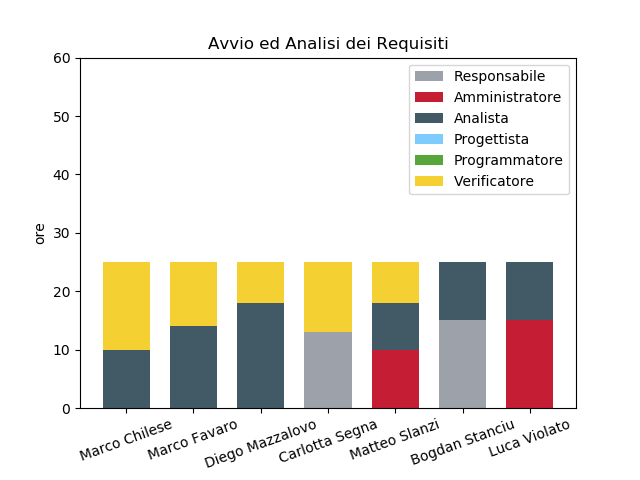
\includegraphics[width=1\linewidth]{./images/fig_aar.png}
  		\caption{Grafico suddivisione ore per persona nel periodo di Avvio ed Analisi dei Requisiti}
  		\label{fig:grafico suddivione ruoli aar}
\end{figure}



\subsubsection{Prospetto economico}
Nel periodo di \textit{Avvio ed Analisi dei Requisiti} la suddivisione oraria, per quanto riguarda i ruoli, è la seguente: 

\begin{longtable}{| C{.30\textwidth}| C{.15\textwidth}| C{.20\textwidth}|}
\hline
\textbf{Ruolo} & \textbf{Ore} & \textbf{Costo in \euro} \\
\hline
Responsabile & 26 & \EUR{780.00} \\
\hline
Amministratore & 23 & \EUR{460.00} \\
\hline
Analista & 69 & \EUR{1725.00} \\
\hline
Progettista & - & - \\
\hline
Programmatore & - & - \\
\hline
Verificatore & 57 & \EUR{855.00}\\
\hline
\textbf{Totale} & 175 & \EUR{3820.00} \\
\hline

\caption{Distribuzione oraria dei ruoli nel periodo di Avvio ed Analisi dei Requisiti}
\label{tab: distribuzione oraria aar}
\end{longtable}

Il seguente grafico dà una rappresentazione visiva della suddivisione nei ruoli:
\begin{figure}[H]
	\centering
  		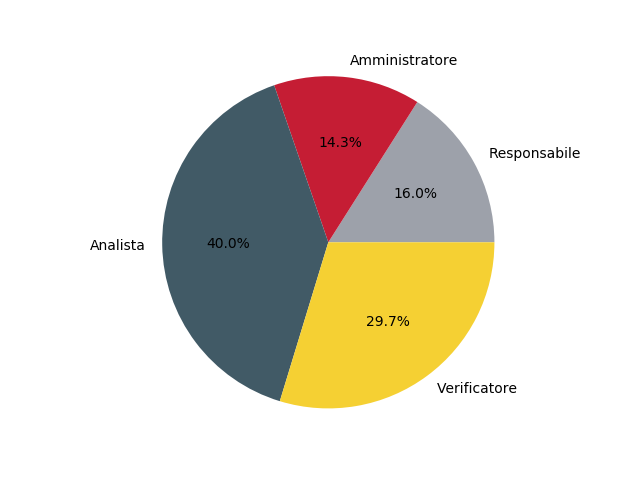
\includegraphics[width=0.8\linewidth]{./images/torta_aar.png}
  		\caption{Grafico suddivisione ruoli nel periodo di Avvio ed Analisi dei Requisiti}
  		\label{fig:grafico suddivione ruoli periodo di Avvio ed analisi dei requisiti}
\end{figure}

\subsection{Risanamento Criticità}
\subsubsection{Prospetto orario}

Nel periodo di \textit{Risanamento Criticità} la suddivisione oraria, per quanto riguarda i ruoli, è la seguente:

\begin{longtable}{|C{.30\textwidth}|C{.06\textwidth}|C{.06\textwidth}|C{.06\textwidth} | C{.06\textwidth}| C{.06\textwidth} | C{.06\textwidth} | C{.10\textwidth} |}
\hline
\textbf{Nome} & \textbf{RE} & \textbf{AM} & \textbf{AN} & \textbf{PJ} & \textbf{PR} & \textbf{VE} & \textbf{Totale}\\
\hline 
Marco Chilese & - & - & - & - & - & 7 & 7 \\
\hline
Marco Favaro & - & - & 7 & - & - & - & 7 \\
\hline
Diego Mazzalovo & - & - & 7 & - & - & - & 7 \\
\hline
Carlotta Segna & - & - & - & - & - & 7 & 7 \\
\hline
Matteo Slanzi & - & - & 7 & - & - & - & 7 \\
\hline
Bogdan Stanciu & 7 & - & - & - & - & - & 7 \\
\hline
Luca Violato & - & 7 & - & - & - & - & 7 \\
\hline

\caption{Distribuzione oraria nel periodo di Risanamento Criticità 1}
\label{Distribuzione oraria del periodo di rc1}
\end{longtable}



Il seguente grafico dà una visione grafica della suddivisione dei ruoli per il periodo di \textit{Risanamento criticità}:
\begin{figure}[H]
  \centering
  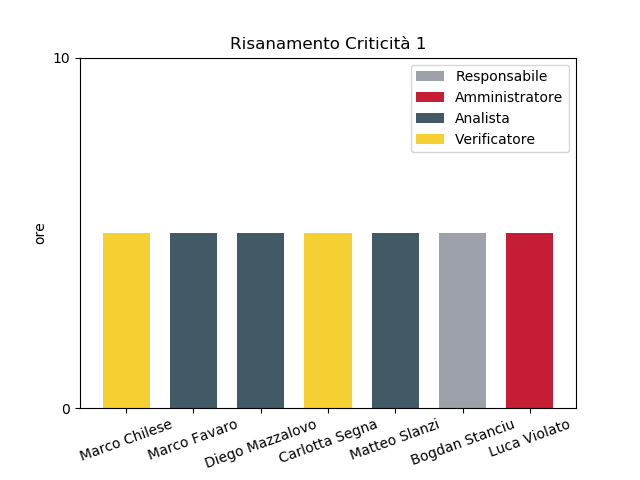
\includegraphics[width=1\linewidth]{./images/fig_rc1.png}
  \caption{Grafico suddivisione ore per persona nel periodo di Risanamento Criticità 1}
  \label{fig:grafico suddivione ruoli rc1}
\end{figure}

\subsubsection{Prospetto economico}
\begin{longtable}{| C{.30\textwidth}| C{.15\textwidth}| C{.20\textwidth}|}
\hline
\textbf{Ruolo} & \textbf{Ore} & \textbf{Costo in \euro} \\
\hline 
Responsabile & 7 & \EUR{210.00} \\
\hline
Amministratore & 7 & \EUR{140.00} \\
\hline
Analista & 21 & \EUR{525.00} \\
\hline
Progettista & - & - \\
\hline
Programmatore & - & - \\
\hline
Verificatore & 14 & \EUR{210.00}\\
\hline
\textbf{Totale} & 49 & \EUR{1085.00} \\
\hline


\caption{Distribuzione oraria dei ruoli nel periodo di Risanamento Criticità 1}
\label{Distribuzione oraria del periodo di rc1}
\end{longtable}

Il seguente grafico dà una rappresentazione visiva della suddivisione nei ruoli:
\begin{figure}[H]
	\centering
  		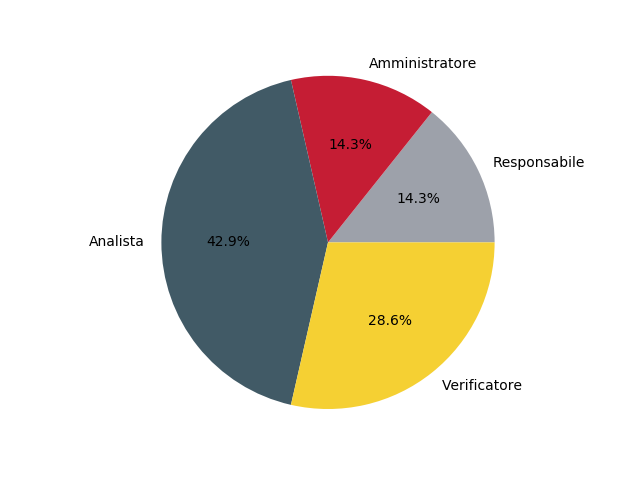
\includegraphics[width=0.8\linewidth]{./images/torta_rc1.png}
  		\caption{Grafico suddivisione ruoli nel periodo di Risanamento Criticità 1}
  		\label{fig:grafico suddivione ruoli periodo di rc1}
\end{figure}


\subsection{Progettazione Architetturale}
\subsubsection{Prospetto orario}

Nel periodo di \textit{Progettazione Architetturale} la suddivisione oraria, per ogni membro del gruppo, è la seguente:


\begin{longtable}{|C{.30\textwidth}|C{.06\textwidth}|C{.06\textwidth}|C{.06\textwidth} | C{.06\textwidth}| C{.06\textwidth} | C{.06\textwidth} | C{.10\textwidth} |}
\hline
\textbf{Nome} & \textbf{RE} & \textbf{AM} & \textbf{AN} & \textbf{PJ} & \textbf{PR} & \textbf{VE} & \textbf{Totale}\\
\hline 
Marco Chilese & - & 10 & - & 7 & 5 & - & 22 \\
\hline
Marco Favaro & 9 & - & 8 & - & - & 5 & 22 \\
\hline
Diego Mazzalovo & 8 & - & - & 7 & 7 & - & 22 \\ 
\hline
Carlotta Segna & - & - & 5 & 5 & 12 & - & 22 \\
\hline
Matteo Slanzi & - & - & 4 & - & 7 & 11 & 22 \\
\hline
Bogdan Stanciu & - & 8 & - & - & 14 & - & 22 \\
\hline
Luca Violato & - & - & 7 & 6 & - & 9 & 22 \\
\hline 

\caption{Distribuzione oraria del periodo di Progettazione Architetturale}
\label{Distribuzione oraria del periodo di pa}
\end{longtable}

Il seguente grafico dà una visione grafica della suddivisione dei ruoli per il periodo di Progettazione Architetturale:

\begin{figure}[H]
	\centering
  		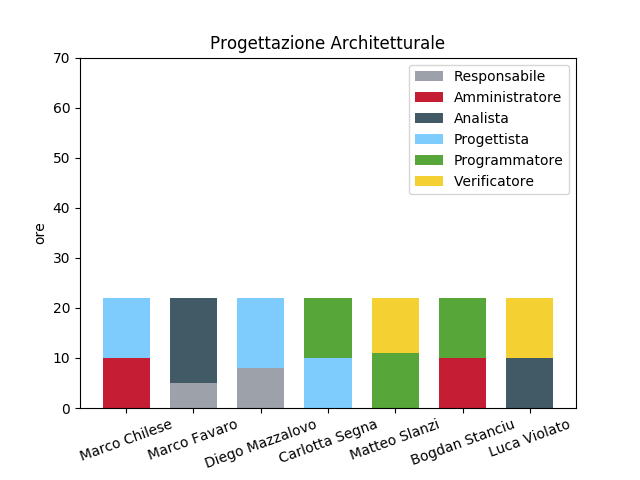
\includegraphics[width=1\linewidth]{./images/fig_pa.png}
  		\caption{Grafico suddivisione ore per persona nel periodo di Progettazione Architetturale}
  		\label{fig:grafico suddivione ruoli periodo di pa}
\end{figure}



\subsubsection{Prospetto economico}
\begin{longtable}{| C{.30\textwidth}| C{.15\textwidth}| C{.20\textwidth}|}
\hline
\textbf{Ruolo} & \textbf{Ore} & \textbf{Costo in \euro} \\
\hline 
Responsabile & 17 & \EUR{510.00} \\
\hline
Amministratore & 18 & \EUR{360.00}\\
\hline
Analista & 24 & \EUR{600.00} \\
\hline
Progettista & 25 & \EUR{550.00} \\
\hline
Programmatore & 45 & \EUR{675.00} \\
\hline
Verificatore & 25 & \EUR{375.00} \\
\hline
\textbf{Totale} & 154 & \EUR{3070.00}\\ 
\hline

\caption{Distribuzione oraria dei ruoli nel periodo di Progettazione Architetturale}
\label{Distribuzione oraria del periodo di pa}
\end{longtable}

Il seguente grafico dà una rappresentazione visiva della suddivisione nei ruoli:
\begin{figure}[H]
	\centering
  		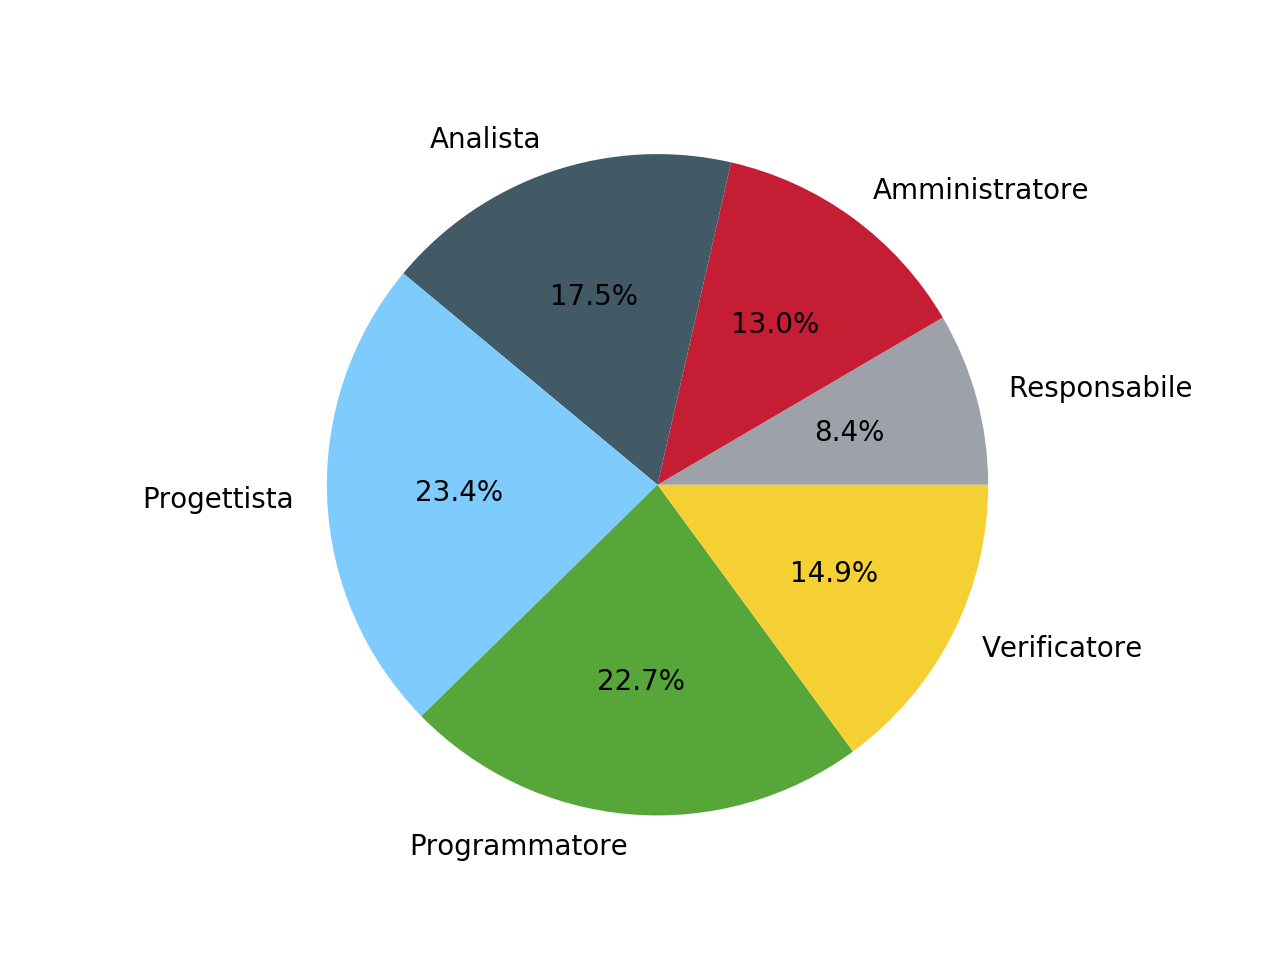
\includegraphics[width=0.8\linewidth]{./images/torta_pa.png}
  		\caption{Grafico suddivisione ruoli nel periodo di Progettazione Architetturale}
  		\label{fig:grafico suddivione ruoli pa}
\end{figure}


\subsection{Risanamento Criticità}
\subsubsection{Prospetto orario}

\begin{longtable}{|C{.30\textwidth}|C{.06\textwidth}|C{.06\textwidth}|C{.06\textwidth} | C{.06\textwidth}| C{.06\textwidth} | C{.06\textwidth} | C{.10\textwidth} |}
\hline
\textbf{Nome} & \textbf{RE} & \textbf{AM} & \textbf{AN} & \textbf{PJ} & \textbf{PR} & \textbf{VE} & \textbf{Totale}\\
\hline 
Marco Chilese & - & 5 & - & - & - & - & 5 \\
\hline
Marco Favaro & 5 & - & - & - & - & - & 5 \\
\hline
Diego Mazzalovo & - & - & - & 5 & - & - & 5 \\
\hline
Carlotta Segna & - & - & - & - & 5 & - & 5 \\
\hline
Matteo Slanzi & - & - & - & - & - & 5 & 5 \\
\hline
Bogdan Stanciu & - & - & 5 & - & - & - & 5 \\
\hline
Luca Violato & - & - & - & - & - & 5 & 5 \\   
\hline


\caption{Distribuzione oraria del periodo di Risanamento Criticità 2}
\label{Distribuzione oraria rc2}
\end{longtable}

Il seguente grafico dà una visione grafica della suddivisione dei ruoli per il periodo di \textit{Risanamento Criticità}:\begin{figure}[H]
	\centering
  		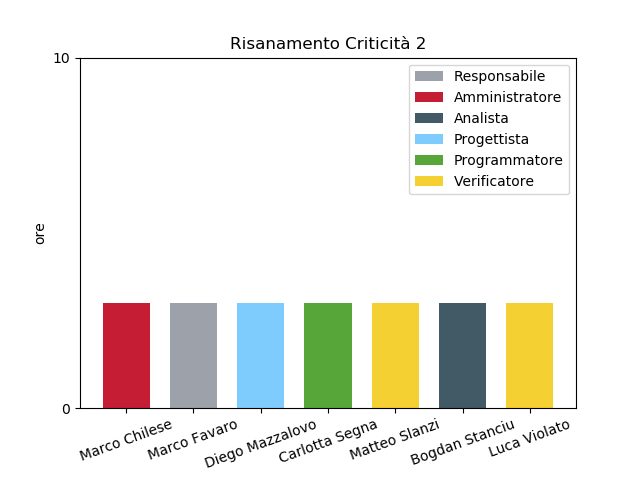
\includegraphics[width=1\linewidth]{./images/fig_rc2.png}
  		\caption{Grafico suddivisione ore per persona nel periodo di Risanamento Criticità 2}
  		\label{fig:grafico suddivione ruoli rc2}
\end{figure}



\subsubsection{Prospetto economico}
\begin{longtable}{| C{.30\textwidth}| C{.15\textwidth}| C{.20\textwidth}|}
\hline
\textbf{Ruolo} & \textbf{Ore} & \textbf{Costo in \euro} \\
\hline 
Responsabile & 5 & \EUR{150.00} \\
\hline
Amministratore & 5 & \EUR{100.00} \\
\hline
Analista & 5 & \EUR{125.00} \\
\hline
Progettista & 5 & \EUR{110.00}\\
\hline
Programmatore & 5 & \EUR{75.00} \\
\hline 
Verificatore & 10 & \EUR{150.00} \\
\hline
\textbf{Totale} & 35 & \EUR{710.00} \\
\hline 

\caption{Distribuzione oraria dei ruoli nel periodo di Risanamento Criticità 2}
\label{Distribuzione oraria rc2}
\end{longtable}

Il seguente grafico dà una rappresentazione visiva della suddivisione nei ruoli:
\begin{figure}[H]
	\centering
  		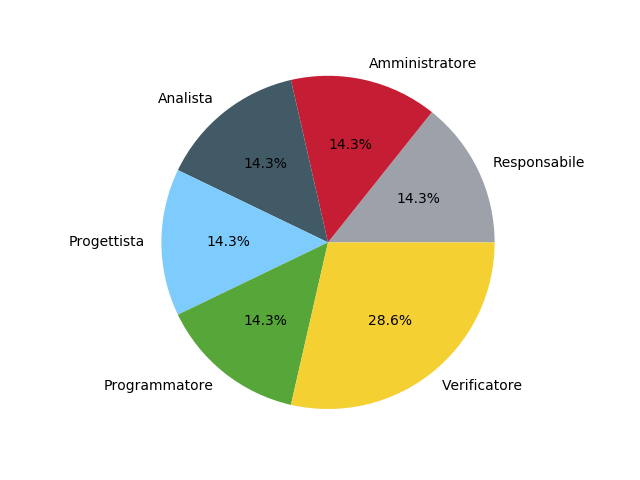
\includegraphics[width=0.8\linewidth]{./images/torta_rc2.png}
  		\caption{Grafico suddivisione ruoli nel periodo di Risanamento Criticità 2}
  		\label{fig:grafico suddivione ruoli rc2}
\end{figure}

\newpage
\subsection{Progettazione di Dettaglio e Codifica}
\subsubsection{Prospetto orario}

Nel periodo di \textit{Progettazione di Dettaglio e Codifica} la suddivisione oraria, per ogni membro del gruppo, è la seguente:

\begin{longtable}{|C{.30\textwidth}|C{.06\textwidth}|C{.06\textwidth}|C{.06\textwidth} | C{.06\textwidth}| C{.06\textwidth} | C{.06\textwidth} | C{.10\textwidth} |}
	\hline
	\textbf{Nome} & \textbf{RE} & \textbf{AM} & \textbf{AN} & \textbf{PJ} & \textbf{PR} & \textbf{VE} & \textbf{Totale}\\
	\hline 
	Marco Chilese & - & - & 8 & 16 & 16 & 10 & 50 \\
	\hline
	Marco Favaro &  - & - & - & 14 & 19 & 17 & 50 \\
	\hline
	Diego Mazzalovo & - & 8 & - & 11 & 20 & 11 & 50 \\
	\hline
	Carlotta Segna & - & 7 & - & 13 & 16 & 14 & 50 \\
	\hline
	Matteo Slanzi & 9 & - & 5 & 18 & 18 & - & 50 \\
	\hline
	Bogdan Stanciu & - & - & 10 & 22 & - & 18 & 50 \\
	\hline
	Luca Violato & 10 & - & - & 10 & 21 & 9 & 50 \\   
	\hline


\caption{Distribuzione oraria nel periodo di Progettazione di Dettaglio e Codifica}
\label{Distribuzione oraria pdc}
\end{longtable}

Il seguente grafico dà una visione grafica della suddivisione dei ruoli per il periodo di \textit{Progettazione di Dettaglio e Codifica}:

\begin{figure}[H]
	\centering
	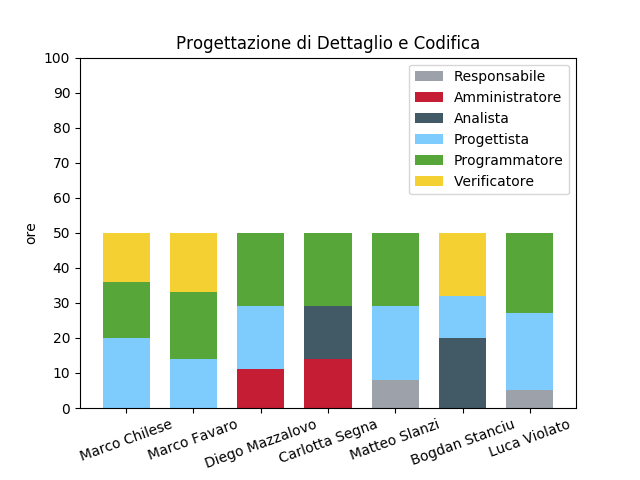
\includegraphics[width=1\linewidth]{./images/fig_pdc.png}
	\caption{Grafico suddivisione ore per persona nel periodo di Progettazione di Dettaglio e Codifica}
	\label{fig:grafico suddivione ruoli periodo pdc}
\end{figure}

\subsubsection{Prospetto economico}
\begin{longtable}{| C{.30\textwidth}| C{.15\textwidth}| C{.20\textwidth}|}
	\hline
	\textbf{Ruolo} & \textbf{Ore} & \textbf{Costo in \euro} \\
	\hline 
	Responsabile & 19 & \EUR{570.00} \\
	\hline
	Amministratore & 15 & \EUR{300.00}\\
	\hline
	Analista & 23 & \EUR{575.00} \\
	\hline
	Progettista & 104 & \EUR{2288.00} \\
	\hline
	Programmatore & 110 & \EUR{1650.00} \\
	\hline
	Verificatore & 79 & \EUR{1185.00} \\
	\hline
	\textbf{Totale} & 350 & \EUR{6568.00}\\ 
	\hline
	
	\caption{Distribuzione oraria del periodo di Progettazione di Dettaglio e Codifica}
	\label{Distribuzione oraria pdc}
\end{longtable}

Il seguente grafico dà una rappresentazione visiva della suddivisione nei ruoli:
\begin{figure}[H]
	\centering
	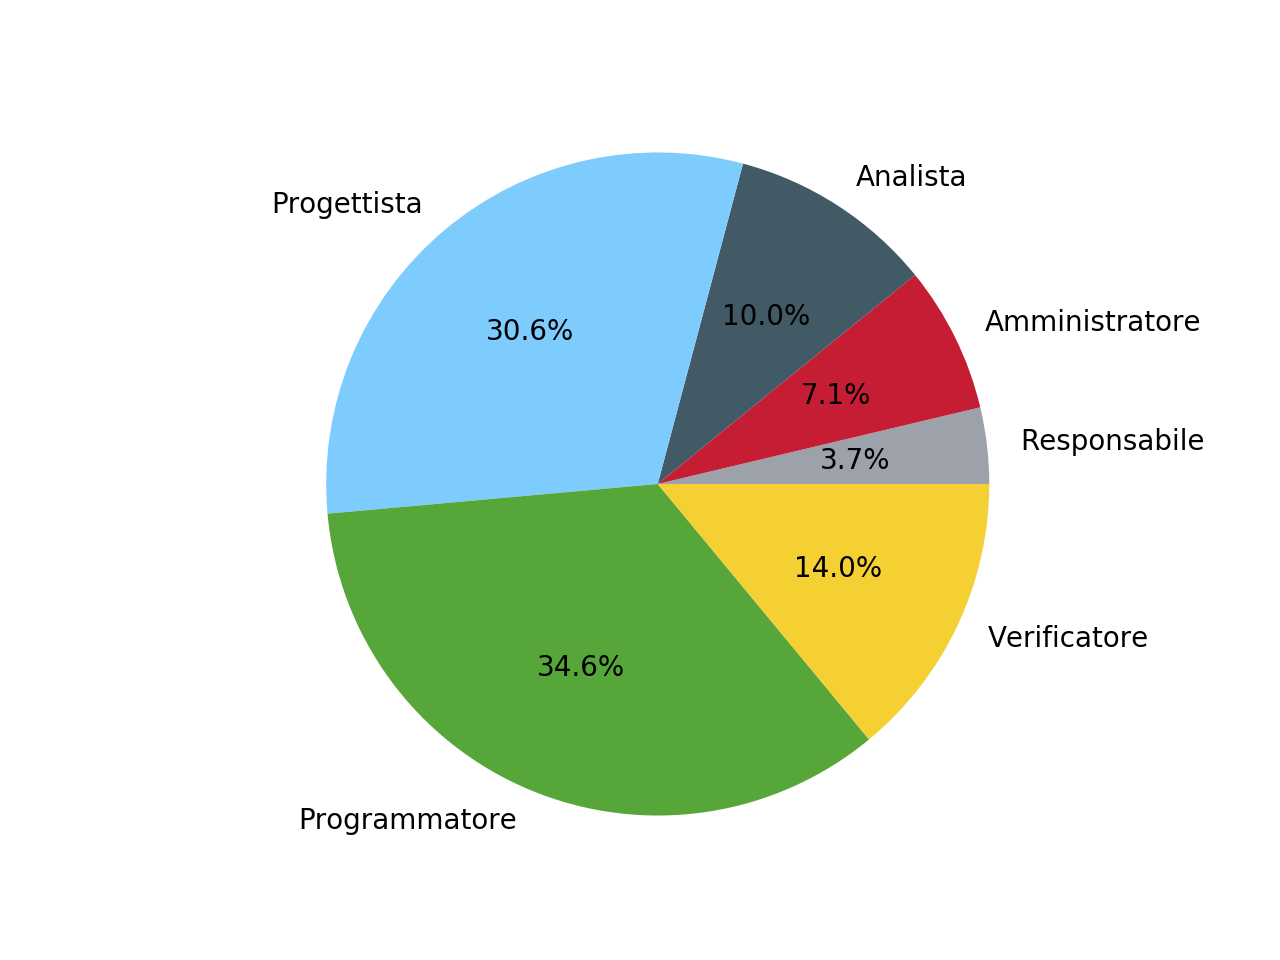
\includegraphics[width=0.8\linewidth]{./images/torta_pdc.png}
	\caption{Grafico suddivisione ore per persona nel periodo di Progettazione di Dettaglio e Codifica}
	\label{fig:grafico suddivione ruoli periodo pdc}
\end{figure}


\subsection{Risanamento Criticità}
\subsubsection{Prospetto orario}
\begin{longtable}{|C{.30\textwidth}|C{.06\textwidth}|C{.06\textwidth}|C{.06\textwidth} | C{.06\textwidth}| C{.06\textwidth} | C{.06\textwidth} | C{.10\textwidth} |}
	\hline
	\textbf{Nome} & \textbf{RE} & \textbf{AM} & \textbf{AN} & \textbf{PJ} & \textbf{PR} & \textbf{VE} & \textbf{Totale}\\
	\hline 
	Marco Chilese & - & - & 4 & - & - & - & 4 \\
	\hline
	Marco Favaro & - & - & - & - & - & 4 & 4 \\
	\hline
	Diego Mazzalovo & - & - & - & - & 4 & - & 4 \\
	\hline
	Carlotta Segna & - & 4 & - & - & - & - & 4 \\
	\hline
	Matteo Slanzi & - & - & - & - & 4 & - & 4 \\
	\hline
	Bogdan Stanciu & - & - & - & 4 & - & - & 4 \\
	\hline
	Luca Violato & 4 & - & - & - & - & - & 4 \\   
	\hline
	
	
	\caption{Distribuzione oraria del periodo di Risanamento Criticità 3}
	\label{Distribuzione oraria rc3}
\end{longtable}

Il seguente grafico dà una visione grafica della suddivisione dei ruoli per il periodo di Risanamento criticità:\begin{figure}[H]
	\centering
	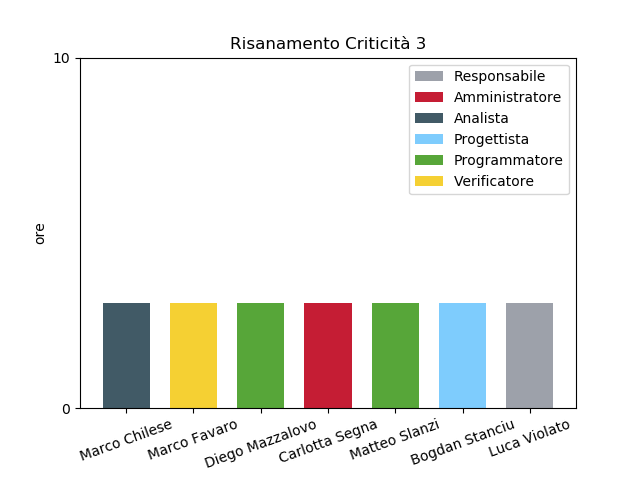
\includegraphics[width=1\linewidth]{./images/fig_rc3.png}
	\caption{Grafico suddivisione ore per persona nel periodo di Risanamento Criticità 3}
	\label{fig:grafico suddivione ruoli rc3}
\end{figure}

\subsubsection{Prospetto economico}
\begin{longtable}{| C{.30\textwidth}| C{.15\textwidth}| C{.20\textwidth}|}
	\hline
	\textbf{Ruolo} & \textbf{Ore} & \textbf{Costo in \euro} \\
	\hline 
	Responsabile & 4 & \EUR{120.00} \\
	\hline
	Amministratore & 4 & \EUR{80.00} \\
	\hline
	Analista & 4 & \EUR{100.00} \\
	\hline
	Progettista & 4 & \EUR{88.00}\\
	\hline
	Programmatore & 8 & \EUR{120.00} \\
	\hline 
	Verificatore & 4 & \EUR{60.00} \\
	\hline
	\textbf{Totale} & 28 & \EUR{568.00} \\
	\hline 


\caption{Distribuzione oraria dei ruoli nel periodo di Risanamento Criticità 3}
\label{Distribuzione oraria rc3}
\end{longtable}

Il seguente grafico dà una visione grafica della suddivisione dei ruoli per il periodo di Risanamento Criticità:\begin{figure}[H]
	\centering
	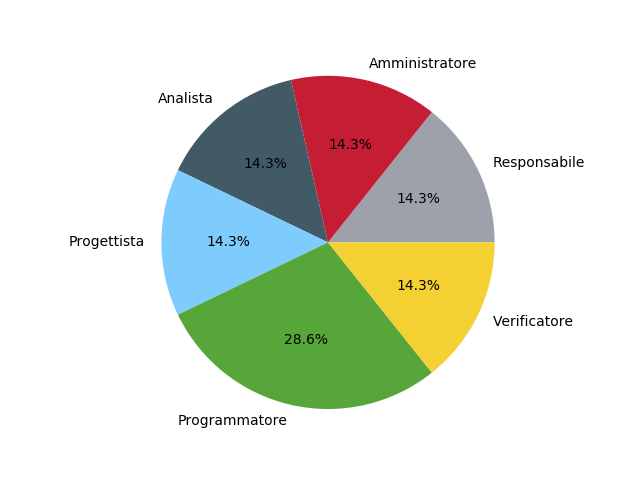
\includegraphics[width=0.8\linewidth]{./images/torta_rc3.png}
	\caption{Grafico suddivisione ruoli nel periodo di Risanamento Criticità 3}
	\label{fig:grafico suddivione ruoli rc3}
\end{figure}

\newpage

\subsection{Validazione e Collaudo}
\subsubsection{Prospetto orario}
Nel periodo di \textit{Validazione e Collaudo} la suddivisione oraria, per ogni membro del gruppo, è la seguente:

\begin{longtable}{|C{.30\textwidth}|C{.06\textwidth}|C{.06\textwidth}|C{.06\textwidth} | C{.06\textwidth}| C{.06\textwidth} | C{.06\textwidth} | C{.10\textwidth} |}
	\hline
	\textbf{Nome} & \textbf{RE} & \textbf{AM} & \textbf{AN} & \textbf{PJ} & \textbf{PR} & \textbf{VE} & \textbf{Totale}\\
	\hline 
	Marco Chilese & 8 & - & - & - & 5 & 9 & 22 \\
	\hline
	Marco Favaro &  - & 11 & - & - & 3 & 8 & 22 \\
	\hline
	Diego Mazzalovo & - & - & - & 6 & 6 & 10 & 22 \\
	\hline
	Carlotta Segna & - & 6 & - & 4 & 5 & 7 & 22 \\
	\hline
	Matteo Slanzi & - & - & - & 7 & 6 & 9 & 22 \\
	\hline
	Bogdan Stanciu & - & - & - & 5 & 8 & 9 & 22 \\
	\hline
	Luca Violato & - & - & - & - & 10 & 12 & 22 \\   
	\hline
	
	
	\caption{Distribuzione oraria nel periodo di Validazione e Collaudo}
	\label{Distribuzione oraria vc}
\end{longtable}

Il seguente grafico dà una visione grafica della suddivisione dei ruoli per il periodo di \textit{Validazione e Collaudo}:

\begin{figure}[H]
	\centering
	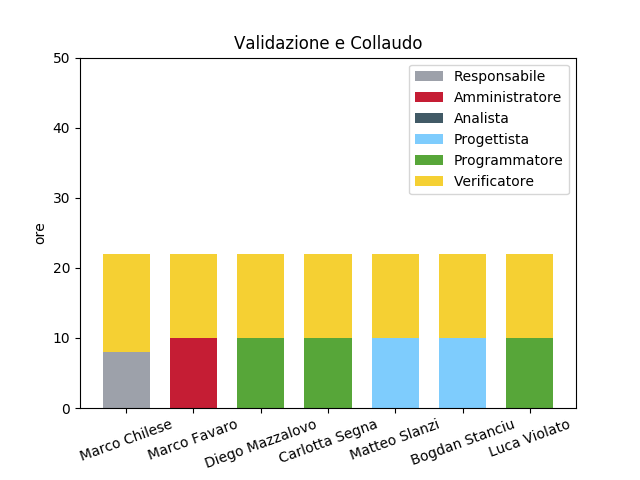
\includegraphics[width=1\linewidth]{./images/fig_vc.png}
	\caption{Grafico suddivisione ore per persona nel periodo di Validazione e Collaudo}
	\label{fig:grafico suddivione ruoli periodo vc}
\end{figure}

\begin{longtable}{| C{.30\textwidth}| C{.15\textwidth}| C{.20\textwidth}|}
	\hline
	\textbf{Ruolo} & \textbf{Ore} & \textbf{Costo in \euro} \\
	\hline 
	Responsabile & 8 & \EUR{240.00} \\
	\hline
	Amministratore & 17 & \EUR{340.00}\\
	\hline
	Analista & 0 & \EUR{0.00} \\
	\hline
	Progettista & 22 & \EUR{484.00} \\
	\hline
	Programmatore & 43 & \EUR{645.00} \\
	\hline
	Verificatore & 64 & \EUR{960.00} \\
	\hline
	\textbf{Totale} & 154 & \EUR{2669.00}\\ 
	\hline
	
	\caption{Distribuzione oraria dei ruoli nel periodo di Validazione e Collaudo}
	\label{Distribuzione oraria del periodo di Validazione e collaudo}
\end{longtable}

Il seguente grafico dà una rappresentazione visiva della suddivisione nei ruoli:
\begin{figure}[H]
	\centering
	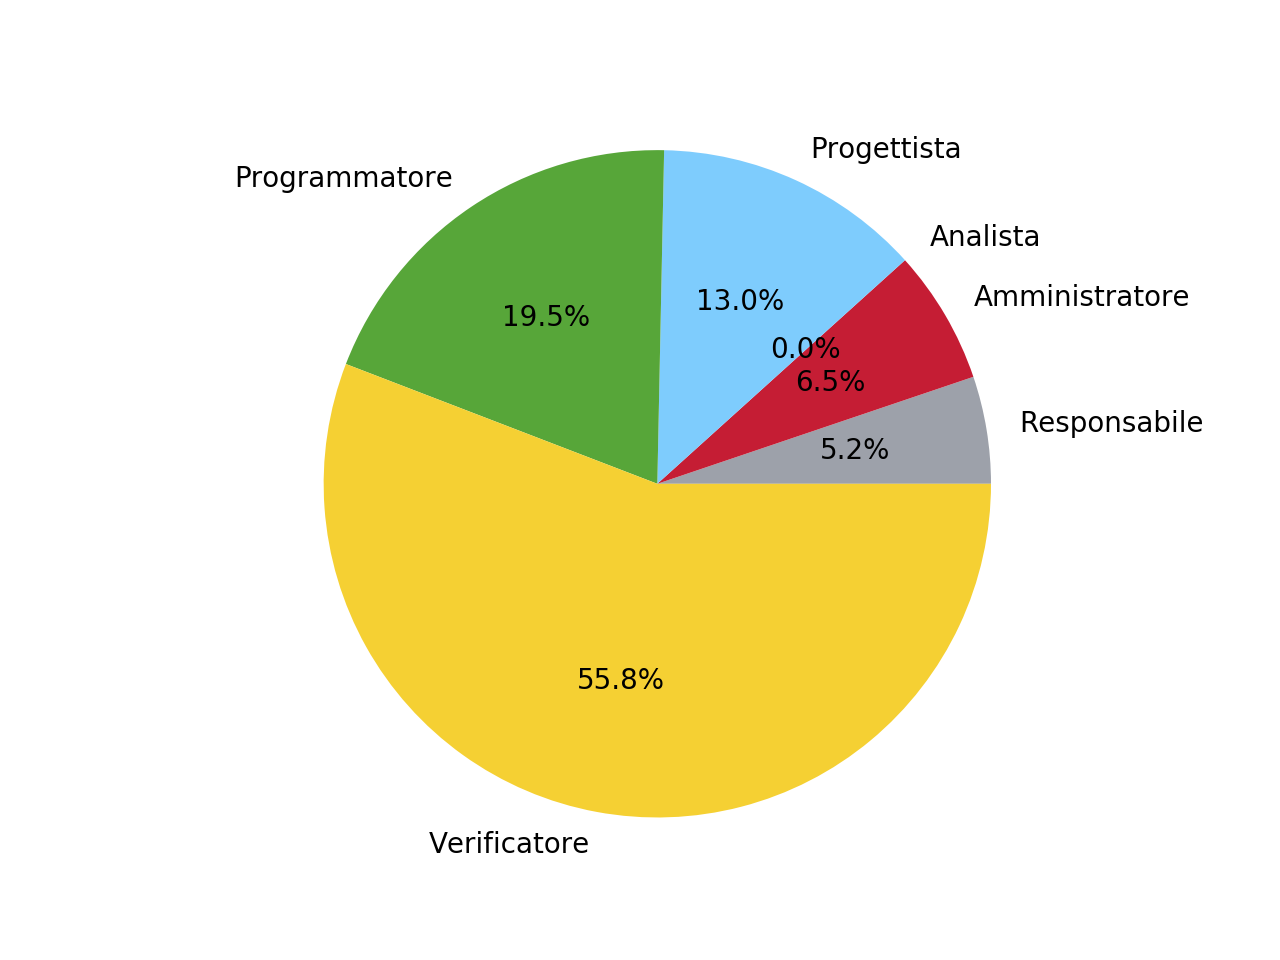
\includegraphics[width=0.8\linewidth]{./images/torta_vc.png}
	\caption{Grafico suddivisione ruoli nel periodo di Validazione e Collaudo}
	\label{fig:grafico suddivione ruoli periodo di Validazione e collaudo}
\end{figure}

\newpage

\subsection{Totale ore rendicontate}
\subsubsection{Prospetto orario}

Le ore di seguito riportate sono da considerarsi a carico del committente, che non includono le ore della prima fase:

\begin{longtable}{|C{.30\textwidth}|C{.06\textwidth}|C{.06\textwidth}|C{.06\textwidth} | C{.06\textwidth}| C{.06\textwidth} | C{.06\textwidth} | C{.10\textwidth} |}
\hline
\textbf{Nome} & \textbf{RE} & \textbf{AM} & \textbf{AN} & \textbf{PJ} & \textbf{PR} & \textbf{VE} & \textbf{Totale}\\
\hline 
Marco Chilese & 8 & 15 & 12 & 23 & 26 & 26 & 110\\
\hline
Marco Favaro & 14 & 11 & 15 & 14 & 22 & 34 & 110\\
\hline
Diego Mazzalovo & 8 & 8 & 7 & 29 & 37 & 21 & 110\\
\hline
Carlotta Segna & - & 17 & 5 & 22 & 38 & 28 & 110\\
\hline
Matteo Slanzi & 9 & - & 16 & 25 & 35 & 25 & 110\\
\hline
Bodgan Stanciu & 7 & 8 & 15 & 31 & 22 & 27 & 110\\
\hline
Luca Violato & 14 & 7 & 7 & 16 & 31 & 35 & 110 \\
\hline

\caption{Distribuzione oraria delle ore rendicontate}
\label{Distribuzione oraria delle ore rendicontate}
\end{longtable}

Il seguente grafico dà una visione grafica della suddivisione dei ruoli per il periodo di Risanamento criticità:%\begin{figure}[H]

\begin{figure}[H]
	\centering
  		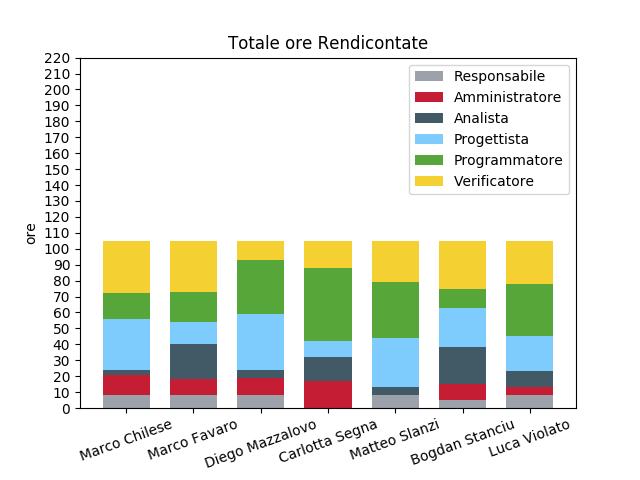
\includegraphics[width=1\linewidth]{./images/fig_tor.png}
  		\caption{Grafico suddivisione ruoli rendicontati.}
  		\label{fig:grafico suddivione ruoli}
\end{figure}


\subsubsection{Prospetto economico}
\begin{longtable}{| C{.30\textwidth}| C{.15\textwidth}| C{.20\textwidth}|}
\hline
\textbf{Ruolo} & \textbf{Ore} & \textbf{Costo in \euro} \\
\hline
Responsabile & 60 & \EUR{1800.00} \\
\hline
Amministratore & 66 & \EUR{1320.00} \\
\hline
Analista & 77 & \EUR{1925.00} \\
\hline
Progettista & 160 & \EUR{3525.00}\\
\hline 
Programmatore & 211 & \EUR{3165.00} \\
\hline
Verificatore & 196 & \EUR{2940.00} \\
\hline 
\textbf{Totale} & 770 & \EUR{14675.00}\\
\hline

\caption{Distribuzione oraria nei ruoli delle ore rendicontate}
\label{Distribuzione oraria a carico del committente}
\end{longtable}

\begin{figure}[H]
	\centering
  		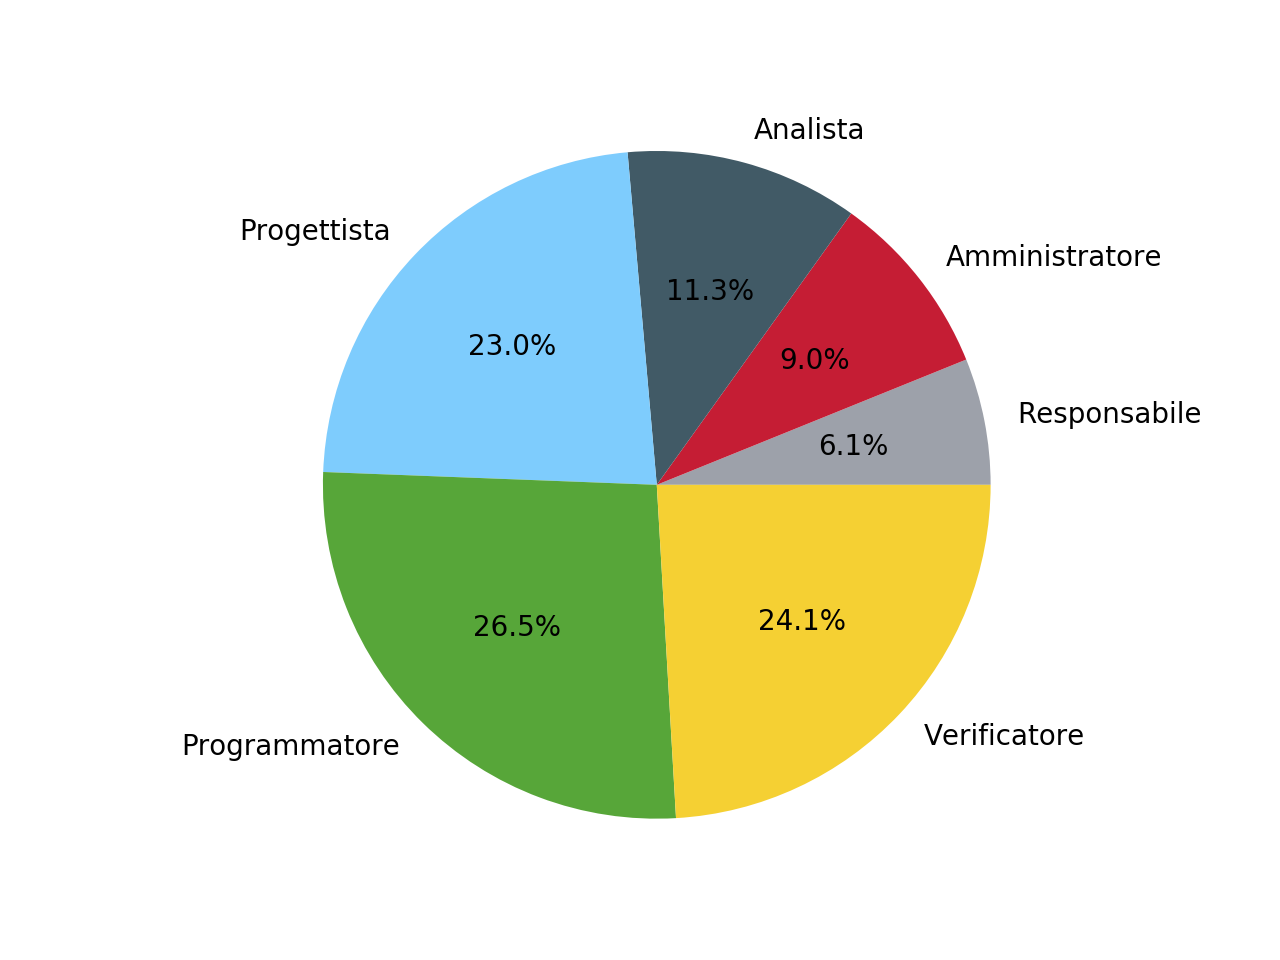
\includegraphics[width=0.8\linewidth]{./images/torta_to.png}
  		\caption{Grafico suddivisione ruoli rendicontati.}
  		\label{fig:grafico suddivione ruoli}
\end{figure}



\subsection{Totale ore con investimento}
\subsubsection{Prospetto orario}


\begin{longtable}{|C{.30\textwidth}|C{.06\textwidth}|C{.06\textwidth}|C{.06\textwidth} | C{.06\textwidth}| C{.06\textwidth} | C{.06\textwidth} | C{.10\textwidth} |}
\hline
\textbf{Nome} & \textbf{RE} & \textbf{AM} & \textbf{AN} & \textbf{PJ} & \textbf{PR} & \textbf{VE} & \textbf{Totale}\\
\hline 
Marco Chilese & 8 & 15 & 22 & 23 & 26 & 41 & 135\\
\hline
Marco Favaro & 14 & 11 & 29 & 14 & 22 & 45 & 135\\
\hline
Diego Mazzalovo & 8 & 8 & 25 & 29 & 37 & 28 & 135\\
\hline
Carlotta Segna & 11 & 17 & 10 & 22 & 38 & 37 & 135\\
\hline
Matteo Slanzi & 9 & 8 & 26 & 25 & 35 & 32 & 135\\
\hline
Bodgan Stanciu & 22 & 8 & 22 & 31 & 22 & 30 & 135\\
\hline
Luca Violato & 14 & 22 & 12 & 16 & 31 & 40 & 135 \\
\hline


\caption{Distribuzione oraria con investimento}
\label{Distribuzione oraria delle ore con investimento}
\end{longtable}

\begin{figure}[H]
	\centering
  		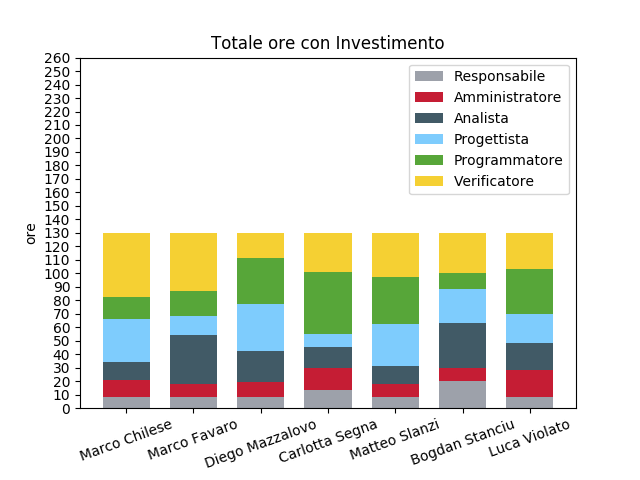
\includegraphics[width=1\linewidth]{./images/fig_toi.png}
  		\caption{Grafico suddivisione ruoli con investimento.}
  		\label{fig:grafico suddivione ruoli con investimento}
\end{figure}

\subsubsection{Prospetto economico}

\begin{longtable}{| C{.30\textwidth}| C{.15\textwidth}| C{.20\textwidth}|}
\hline
\textbf{Ruolo} & \textbf{Ore} & \textbf{Costo in \euro} \\
\hline 
Responsabile & 86 & \EUR{2580.00}\\
\hline
Amministratore & 89 & \EUR{1780.00} \\
\hline
Analista & 146 & \EUR{2190.00} \\
\hline 
Progettista & 160 & \EUR{3520.00}\\
\hline
Programmatore & 211 & \EUR{3570.00} \\
\hline
Verificatore & 253 & \EUR{3165.00} \\
\hline
\textbf{Totale} & 945 & \EUR{16805.00} \\
\hline
\caption{Distribuzione oraria dei ruoli con investimento}
\label{Distribuzione oraria ruoli con investimento}
\end{longtable}

\begin{figure}[H]
	\centering
  		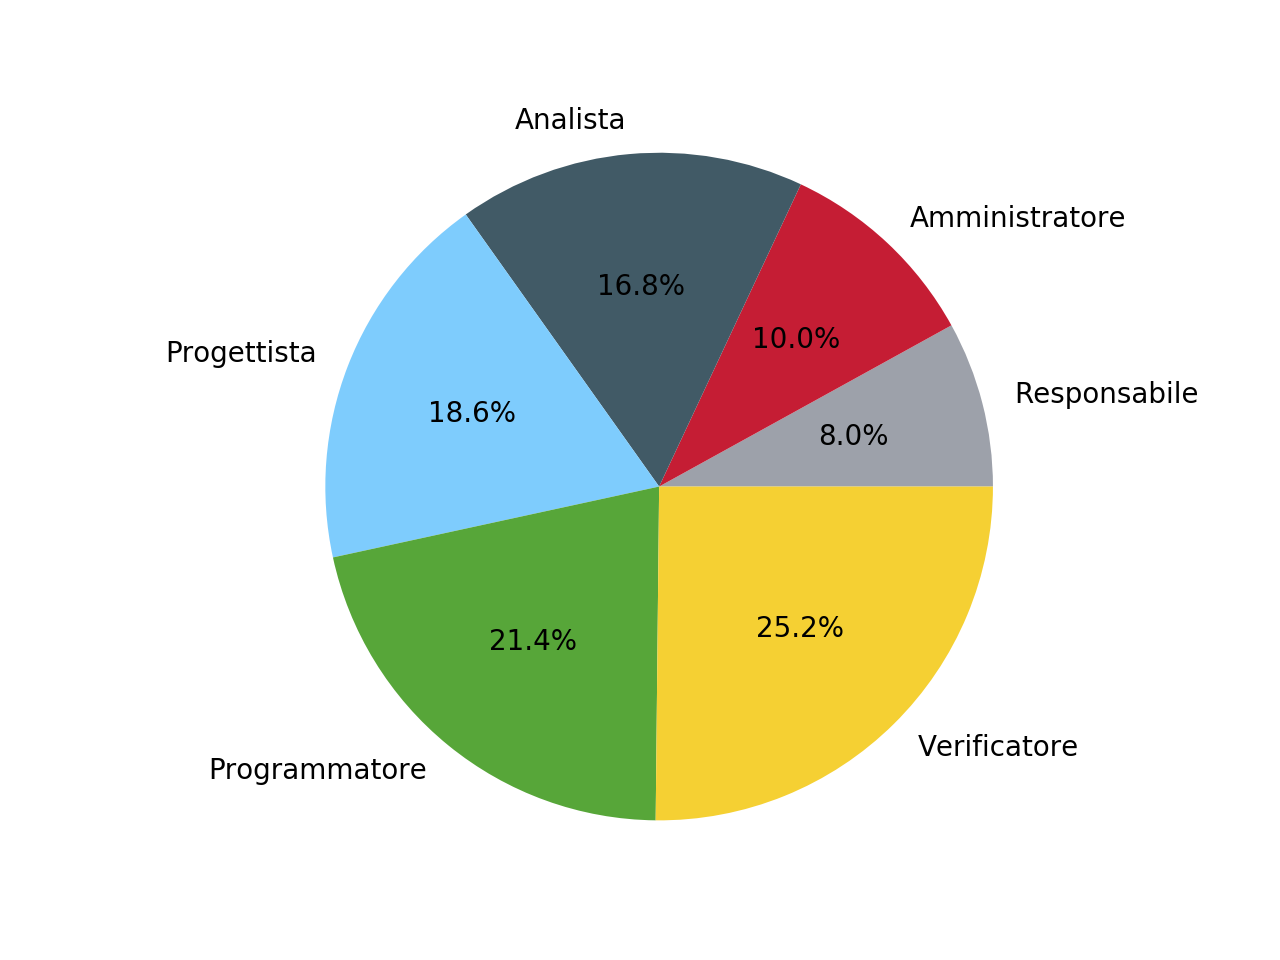
\includegraphics[width=0.8\linewidth]{./images/torta_toci.png}
  		\caption{Grafico suddivisione ruoli con investimento.}
  		\label{fig:grafico suddivione ruoli con investimento}
\end{figure}





\pagebreak

\section{Consuntivo di Periodo e Preventivo a Finire}
\label{CFPPAF}

In questa sezione stiliamo un rendiconto delle attività svolte fino ad ora, al fine di poter confrontare il preventivo stilato con l'effettivo numero di ore svolte da ogni membro del gruppo per ogni periodo.\\
Incrementeremo questa sezione alla fine di ogni periodo.\\
Inseriremo il conteggio in una tabella, così da rendere meglio visibili ore preventivate ed ore effettivamente svolte.\\
Rappresenteremo le prime con un semplice numero, mentre le seconde tra parentesi graffe, seguendo i criteri qui sotto riportati:
\begin{itemize}
	\item \textbf{Positivi}: sono state necessarie più ore di quelle preventivate;
	\item \textbf{Negativi}: sono state necessarie meno ore di quelle preventivate;
	\item \textbf{Invariato}: qualora le ore non dovessero cambiare, verrà semplicemente inserito il numero di ore preventivato.	
\end{itemize}

Inoltre, aggiorneremo anche i dati dei preventivi andando a uniformarli con le ore effettivamente utilizzate durante la fase.\\
Questo ricalcolo è utile solamente al fine di poter verificare la qualità delle attività svolte dal gruppo e non andrà in alcun modo a variare i costi preventivati per la committente.

\newpage

\subsection{Consuntivo di Periodo}
\label{CFP}
\subsubsection{Revisione dei Requisiti}

\paragraph{Prospetto Orario} \-\\

\begin{longtable}{|C{.30\textwidth}|C{.06\textwidth}|C{.06\textwidth}|C{.06\textwidth} | C{.06\textwidth}| C{.06\textwidth} | C{.06\textwidth} | C{.10\textwidth} |}
\hline
\rowcolor{bluelogo}	\textbf{\textcolor{white}{Nome}} & \textbf{\textcolor{white}{RE}} & \textbf{\textcolor{white}{AM}} & \textbf{\textcolor{white}{AN}} & \textbf{\textcolor{white}{PJ}} & \textbf{\textcolor{white}{PR}} & \textbf{\textcolor{white}{VE}} & \textbf{\textcolor{white}{Totale}}\\
\hline 
Marco Chilese & - & - & 10 \{+5\} & - & - & 15 \{-4\} & 25 \{+1\} \\
\hline
\rowcolor{grigio}Marco Favaro & - & - & 14 \{-3\} & - & - & 11 \{+4\} & 25 \{+1\} \\
\hline
Diego Mazzalovo & - & - & 18 \{-5\} & - & - & 7 \{+6\} & 25 \{+1\} \\
\hline
\rowcolor{grigio}Carlotta Segna & 13 \{+3\} & - & - & - & - & 12 \{-2\} & 25 \{+1\} \\
\hline
Matteo Slanzi & - & 10 \{-3\} & 8 \{+4\} & - & - & 7 & 25 \{+1\} \\
\hline
\rowcolor{grigio}Bogdan Stanciu & 15 \{-3\} & - & 10 \{+4\} & - & - & - & 25 \{+1\}\\
\hline
Luca Violato & - & 15 \{+3\} & 10 \{-2\} & - & - & - & 25 \{+1\} \\
\hline


\caption{Consuntivo di Periodo: Avvio ed Analisi dei Requisiti}
\label{tab:cfp_aar}
\end{longtable}

\paragraph{Prospetto Economico} \-\\

\begin{longtable}{| C{.30\textwidth}| C{.15\textwidth}| C{.20\textwidth}|}
\hline
\rowcolor{bluelogo}\textbf{\textcolor{white}{Ruolo}} & \textbf{\textcolor{white}{Ore}} & \textbf{\textcolor{white}{Costo in \euro}} \\
\hline
Responsabile & 28 & \EUR{840.00} \\
\hline
\rowcolor{grigio}Amministratore & 25 & \EUR{500.00} \\
\hline
Analista & 73 \{+3\} & \EUR{1825.00} \{+\EUR{75.00}\}\\
\hline
\rowcolor{grigio}Progettista & - & - \\
\hline
Programmatore & - & - \\
\hline
\rowcolor{grigio}Verificatore & 56 \{+4\} & \EUR{840.00} \{+\EUR{60.00}\}\\
\hline
\textbf{Totale} & 182 \{+7\}& \EUR{4005.00} \{+\EUR{135.00}\}\\
\hline
\caption{Consuntivo di Periodo dei Ruoli: Avvio ed Analisi dei Requisiti}
\label{tab:doaar}
\end{longtable}

\paragraph{Variazioni nella Pianificazione} ~\\
Durante lo svolgimento delle attività non sono state commessi ritardi, quindi la pianificazione è rimasta invariata.


\paragraph{Conclusioni} \-\\
Il numero di ore preventivato differisce da quelle realmente utilizzate in quanto, approcciandosi ad un nuovo modo di svolgere un progetto, non siamo stati in grado di preventivare correttamente il numero di ore che si sarebbero poi andate, effettivamente, ad utilizzare. Ciò è dovuto al fatto che siano state utilizzate più ore, rispetto a quanto preventivato, per la stesura del \textit{Piano di Progetto v1.0.0}, andando così ad aumentare le ore di \textit{Responsabile}. Un discorso equivalente può essere effettuato per il ruolo di \textit{Analista} , in quanto il documento \textit{Analisi dei Requisiti v1.0.0} ha richiesto un'analisi più lunga ed approfondita di quanto precedentemente preventivato. \\
Il \textit{Verificatore} ha necessitato più ore in quanto i documenti sono stati rivisti più volte, al fine di controllare le modifiche che venivano effettuate. \\
Alla fine di questo periodo il numero si è quindi verificato un incremento di 7 ore totali, andando ad aggiungere \EUR{135.00} al costo totale della prima fase, a carico del gruppo. 

\subsubsection{Risanamento Criticità}
\label{RA1}

\paragraph{Prospetto Orario} \-\\

\begin{longtable}{|C{.30\textwidth}|C{.06\textwidth}|C{.06\textwidth}|C{.06\textwidth} | C{.06\textwidth}| C{.06\textwidth} | C{.06\textwidth} | C{.10\textwidth} |}
\hline
\rowcolor{bluelogo}	\textbf{\textcolor{white}{Nome}} & \textbf{\textcolor{white}{RE}} & \textbf{\textcolor{white}{AM}} & \textbf{\textcolor{white}{AN}} & \textbf{\textcolor{white}{PJ}} & \textbf{\textcolor{white}{PR}} & \textbf{\textcolor{white}{VE}} & \textbf{\textcolor{white}{Totale}}\\
\hline \hline

Marco Chilese & - & - & - & - & - & 3 \{-2\} & 3 \{-2\}\\
\hline
\rowcolor{grigio}Marco Favaro & - & - & 4 \{-1\} & - & - & - & 4 \{-1\} \\
\hline
Diego Mazzalovo & - & - & 4 \{-1\} & - & - & - & 4 \{-1\} \\
\hline
\rowcolor{grigio}Carlotta Segna & - & - & - & - & - & 3 \{-2\} & 3 \{-2\}\\
\hline
Matteo Slanzi & - & - & 2 \{-3\} & - & - & - & 2 \{-3\}\\
\hline
\rowcolor{grigio}Bogdan Stanciu & 3 \{-2\} & - & - & - & - & - & 3 \{-2\} \\
\hline
Luca Violato & - & 3 \{-2\}& - & - & - & - & 3 \{-2\} \\
\hline

\caption{Consuntivo di Periodo: Risanamento Criticità 1}
\label{Distribuzione oraria del periodo di rc1}
\end{longtable}

\paragraph{Prospetto Economico} \-\\

\begin{longtable}{| C{.30\textwidth}| C{.15\textwidth}| C{.20\textwidth}|}
\hline
\rowcolor{bluelogo}\textbf{\textcolor{white}{Ruolo}} & \textbf{\textcolor{white}{Ore}} & \textbf{\textcolor{white}{Costo in \euro}} \\
\hline 
Responsabile & 3 \{-2\} & \EUR{90.00} \{-\EUR{60.00}\}\\
\hline
\rowcolor{grigio}Amministratore & 3 \{-2\} & \EUR{60.00} \{-\EUR{40.00}\} \\
\hline
Analista & 10 \{-5\} & \EUR{250.00} \{-\EUR{125.00}\} \\
\hline
\rowcolor{grigio}Progettista & - & - \\
\hline
Programmatore & - & - \\
\hline
\rowcolor{grigio}Verificatore & 6 \{-4\} & \EUR{90.00} \{-\EUR{60.00}\}\\
\hline
\textbf{Totale} & 23 \{-12\} & \EUR{490.00} \{-\EUR{285.00}\} \\
\hline
\caption{Consuntivo di Periodo dei ruoli: Risanamento Criticità 1}
\label{Distribuzione oraria Ruoli del Periodo di rc1}
\end{longtable}

\paragraph{Variazioni nella Pianificazione} ~\\
Durante lo svolgimento delle attività non sono state commessi ritardi, quindi la pianificazione è rimasta invariata. \\

\paragraph{Conclusioni} ~\\

Durante il periodo di \textit{Risanamento Criticità}, il monte orario preventivato si è dimostrato superiore alle reali necessità. Durante il periodo sono stati corretti gli errori segnalati alla fine del periodo precedente. Le correzioni si sono svolte sulla documentazione contenente errori. Un impegno maggiore è stato richiesto dal documento \textit{Analisi dei Requisiti v1.0.0}, corretto dagli \textit{Analisti}. \\

\newpage

\subsubsection{Progettazione Architetturale}
\label{pa}

\paragraph{Prospetto Orario} ~\\

\begin{longtable}{|C{.30\textwidth}|C{.06\textwidth}|C{.06\textwidth}|C{.06\textwidth} | C{.06\textwidth}| C{.06\textwidth} | C{.06\textwidth} | C{.10\textwidth} |}
\hline
\rowcolor{bluelogo}	\textbf{\textcolor{white}{Nome}} & \textbf{\textcolor{white}{RE}} & \textbf{\textcolor{white}{AM}} & \textbf{\textcolor{white}{AN}} & \textbf{\textcolor{white}{PJ}} & \textbf{\textcolor{white}{PR}} & \textbf{\textcolor{white}{VE}} & \textbf{\textcolor{white}{Totale}}\\
\hline 
Marco Chilese & - & 12 \{+2\} & - & 12 & - & - & 24 \{+2\} \\
\hline
\rowcolor{grigio}Marco Favaro & 5 & - & 18 \{+1\}  & - & - & - & 23 \{+1\} \\
\hline
Diego Mazzalovo & 6 \{-2\}& - & - & 17 \{+3\} & - & - & 23 \{+1\} \\ 
\hline
\rowcolor{grigio}Carlotta Segna & - & - & - & 10 & 13 \{+1\} & - & 23 \{+1\} \\
\hline
Matteo Slanzi & - & - & - & - & 7 \{-4\} & 9 \{-2\} & 16 \{-6\} \\
\hline
\rowcolor{grigio}Bogdan Stanciu & - & 8 \{-2\}& - & - & 15 \{+3\} & - & 23 \{+1\} \\
\hline
Luca Violato & - & - & 11 \{+1\} & - & - & 14 \{+2\} & 25 \{+3\} \\
\hline 

\caption{Consuntivo di Periodo: Progettazione Architetturale}
\label{Distribuzione oraria del periodo di pa}
\end{longtable}


\paragraph{Prospetto Economico} ~\\

\begin{longtable}{| C{.30\textwidth}| C{.15\textwidth}| C{.20\textwidth}|}
\hline
\rowcolor{bluelogo}\textbf{\textcolor{white}{Ruolo}} & \textbf{\textcolor{white}{Ore}} & \textbf{\textcolor{white}{Costo in \euro}} \\
\hline 
Responsabile & 11 \{-2\}& \EUR{330.00} \{-\EUR{60.00}\} \\
\hline
\rowcolor{grigio}Amministratore & 20 & \EUR{400.00} \\
\hline
Analista & 29 \{+2\} & \EUR{725.00} \{+\EUR{50.00}\}\\
\hline
\rowcolor{grigio}Progettista & 39 \{+3\} & \EUR{858.00} \{+\EUR{66.00}\}\\
\hline
Programmatore & 35 & \EUR{525.00} \\
\hline
\rowcolor{grigio}Verificatore & 23 & \EUR{345.00}\\
\hline
\textbf{Totale} & 157 \{+3\} & \EUR{3183.00} \{+\EUR{56.00}\}\\ 
\hline

\caption{Consuntivo di Periodo dei Ruoli: Progettazione Architetturale}
\label{Distribuzione oraria per ruoli del periodo di pa}
\end{longtable}

\paragraph{Variazioni nella Pianificazione} ~\\
Durante lo svolgimento delle attività non sono state commessi ritardi, quindi la pianificazione è rimasta invariata. \\

\paragraph{Conclusioni} ~\\
L'incremento del documento \textit{Analisi dei Requisiti v2.0.0}, ha richiesto un numero di ore maggiore da parte degli \textit{Analisti} per il suo incremento. L'utilizzo di nuovo tecnologie ha portato gli \textit{Amministratori}, che avevano già una precedente conoscenza di queste. La preparazione del \textit{PoC} ha richiesto maggior tempo rispetto a quanto preventivato e, quindi, le ore di \textit{Programmatori} e \textit{Progettisti} sono aumentate. 

\subsubsection{Risanamento Criticità}
\label{RA2}

\paragraph{Prospetto Orario} \-\\

\begin{longtable}{|C{.30\textwidth}|C{.06\textwidth}|C{.06\textwidth}|C{.06\textwidth} | C{.06\textwidth}| C{.06\textwidth} | C{.06\textwidth} | C{.10\textwidth} |}
\hline
\rowcolor{bluelogo}	\textbf{\textcolor{white}{Nome}} & \textbf{\textcolor{white}{RE}} & \textbf{\textcolor{white}{AM}} & \textbf{\textcolor{white}{AN}} & \textbf{\textcolor{white}{PJ}} & \textbf{\textcolor{white}{PR}} & \textbf{\textcolor{white}{VE}} & \textbf{\textcolor{white}{Totale}}\\
\hline \hline

Marco Chilese & - & - & - & 3 & - & - & 3\\
\hline
\rowcolor{grigio}Marco Favaro & 3 & - & - & - & - & - & 3 \\
\hline
Diego Mazzalovo & - & - & - & 3 & - & - & 3 \\
\hline
\rowcolor{grigio}Carlotta Segna & - & - & - & - & 3 & - & 3\\
\hline
Matteo Slanzi & - & - & - & - & - & 3 & 3\\
\hline
\rowcolor{grigio}Bogdan Stanciu & - & 3 & - & - & - & - & 3 \\
\hline
Luca Violato & - & - & 3 & - & - & - & 3 \\
\hline

\caption{Consuntivo di Periodo: Risanamento Criticità 2}
\label{Distribuzione oraria del periodo di rc2}
\end{longtable}

\paragraph{Prospetto Economico} \-\\

\begin{longtable}{| C{.30\textwidth}| C{.15\textwidth}| C{.20\textwidth}|}
	\hline
	\rowcolor{bluelogo}\textbf{\textcolor{white}{Ruolo}} & \textbf{\textcolor{white}{Ore}} & \textbf{\textcolor{white}{Costo 	in \euro}} \\
	\hline 
	Responsabile & 3 & \EUR{90.00} \\
	\hline
	\rowcolor{grigio}Amministratore & 3 & \EUR{60.00} \\
	\hline
	Analista & 3 & \EUR{75.00} \\
	\hline
	\rowcolor{grigio}Progettista & 3 & \EUR{66.00}\\
	\hline
	Programmatore & 6 & \EUR{90.00} \\
	\hline 
	\rowcolor{grigio}Verificatore & 3 & \EUR{45.00} \\
	\hline
	\textbf{Totale} & 21 & \EUR{426.00} \\
	\hline 

\caption{Consuntivo di Periodo dei ruoli: Risanamento Criticità 2}
\label{Distribuzione ruoli RC2}
\end{longtable}

\paragraph{Variazioni nella Pianificazione} ~\\
Durante lo svolgimento delle attività non sono state commessi ritardi, quindi la pianificazione è rimasta invariata.

\paragraph{Conclusioni} ~\\

Le ore preventivate per questa fase sono state precedentemente correttamente preventivate. Le modifiche apportate sono state quelle segnalate in Revisione di Pianificazione dalla committente. 

\pagebreak

\subsubsection{Progettazione di Dettaglio e Codifica}
\label{PPDC}
\paragraph{Prospetto Orario } ~\\
\begin{longtable}{|C{.30\textwidth}|C{.06\textwidth}|C{.06\textwidth}|C{.06\textwidth} | C{.06\textwidth}| C{.06\textwidth} | C{.06\textwidth} | C{.10\textwidth} |}
	\hline
	\rowcolor{bluelogo}	\textbf{\textcolor{white}{Nome}} & \textbf{\textcolor{white}{RE}} & \textbf{\textcolor{white}{AM}} & \textbf{\textcolor{white}{AN}} & \textbf{\textcolor{white}{PJ}} & \textbf{\textcolor{white}{PR}} & \textbf{\textcolor{white}{VE}} & \textbf{\textcolor{white}{Totale}}\\
	\hline 
	Marco Chilese & - & - & - & 20 & 13 \{-3\} & 17 \{+3\}& 50 \\
	\hline
	\rowcolor{grigio}Marco Favaro &  - & - & - & 14 & 19 \{+4\} & 17 \{-4\} & 50 \\
	\hline
	Diego Mazzalovo & - & 8 \{-3\} & - & 18 & 13 \{-8\} & 11 \{+11\} & 50 \\
	\hline
	\rowcolor{grigio}Carlotta Segna & - & 14 \{-4\} & 15 \{+4\} & - & 21 & - & 50 \\
	\hline
	Matteo Slanzi & 8 & - & - & 11 \{-10\} & 21 & 10 \{+10\} & 50 \\
	\hline
	\rowcolor{grigio}Bogdan Stanciu & - & - & 8 \{-12\} & 12 &  20 \{+20\} & 10 \{-8\} & 50 \\
	\hline
	Luca Violato & 5 & - & - & 22 \{+3\} & 23 \{-3\} & - & 50 \\   
	\hline


\caption{Consuntivo di Periodo dei Ruoli: Progettazione di Dettaglio e Codifica}
\label{CP PDC}
\end{longtable}

\paragraph{Prospetto Economico} ~\\

\begin{longtable}{| C{.30\textwidth}| C{.15\textwidth}| C{.20\textwidth}|}
	\hline
	\rowcolor{bluelogo}\textbf{\textcolor{white}{Ruolo}} & \textbf{\textcolor{white}{Ore}} & \textbf{\textcolor{white}{Costo 	in \euro}} \\
	\hline 
	Responsabile & 13 & \EUR{390.00} \\
	\hline
	\rowcolor{grigio}Amministratore & 22 \{-3\} & \EUR{440.00}  \{-\EUR{60.00}\}\\
	\hline
	Analista & 23 \{-12\}& \EUR{575.00} \{-\EUR{300}\} \\
	\hline
	\rowcolor{grigio}Progettista & 97 \{-10\} & \EUR{2134.00}  \{-\EUR{220.00}\}\\
	\hline
	Programmatore & 130 \{+9\} & \EUR{1950.00} \{+\EUR{135.00\}} \\
	\hline 
	\rowcolor{grigio}Verificatore & 65 \{+16\} & \EUR{975.00} \{+\EUR{240.00\}}\\
	\hline
	\textbf{Totale} & 350 & \EUR{6464.00} \{-\EUR{205.00 }\}\\
	\hline 

\caption{Consuntivo di Periodo dei ruoli: Progettazione di Dettaglio e Codifica}
\label{Distribuzione ruoli pdc}
\end{longtable}

\paragraph{Variazioni nella Pianificazione} ~\\
Durante lo svolgimento delle attività non sono state commessi ritardi, quindi la pianificazione è rimasta invariata.

\paragraph{Conclusioni} ~\\
Nonostante le ore assegnate a ciascuna persona siano, nel totale, rimaste invariate, il numero di ore suddiviso tra persona ha subito delle modifiche. Questo si è verificato in quanto persone con più esperienza sono state assegnate allo svolgimento di compiti con i quali avevano precedentemente familiarizzato. \\
Un aumento delle ore di \textit{Verificatore} è dovuto al continuo controllo di documenti e codice che venivano scritti e sviluppati al fine di annullare gli errori che venivano commessi durante lo sviluppo di questi. L'aumento delle ore del \textit{Programmatore} è dovuto ad un lavoro maggiore rispetto a quanto preventivato. \\
Nella prossima fase vi sarà un incremento minimo dei documenti \textit{Piano di progetto}, \textit{Glossario}, \textit{Norme di Progetto} e \textit{Analisi dei Requisiti}, mentre per quanto riguarda il documento \textit{Piano di Qualifica} ci sarà un incremento notevole che sarà comportato dall'aggiunta di nuovi test di unità. Ci sarà quindi un grosso carico di lavoro per i \textit{Verificatori} che dovranno verificare tutti i documenti e implementare i test di unità e di integrazione precedentemente pianificati. L'esperienza da noi acquisita ci metterà nelle condizioni di non sforare le ore preventivate attuando metodologie di collaborazione tra chi ha scritto il codice e chi dovrà implementare i test. Per quanto riguarda i manuali, eventuali criticità saranno risanate nel minor tempo possibile, e successivamente verrà eseguito un eventuale incremento comportato dall'implementazione di requisiti non obbligatori, con l'obiettivo di rendere il prodotto più appetibile e utilizzabile.\\

\pagebreak

\subsubsection{Risanamento Criticità}
\label{RA3}
\paragraph{Prospetto Orario} \-\\
\begin{longtable}{|C{.30\textwidth}|C{.06\textwidth}|C{.06\textwidth}|C{.06\textwidth} | C{.06\textwidth}| C{.06\textwidth} | C{.06\textwidth} | C{.10\textwidth} |}
	\hline
	\rowcolor{bluelogo}	\textbf{\textcolor{white}{Nome}} & \textbf{\textcolor{white}{RE}} & \textbf{\textcolor{white}{AM}} & \textbf{\textcolor{white}{AN}} & \textbf{\textcolor{white}{PJ}} & \textbf{\textcolor{white}{PR}} & \textbf{\textcolor{white}{VE}} & \textbf{\textcolor{white}{Totale}}\\
	\hline \hline
	
	Marco Chilese & - & - & 5 \{+2\} & - & - & - & 5 \{+2\}\\
	\hline
	\rowcolor{grigio}Marco Favaro & - & - & - & - & - & 3 & 3 \\
	\hline
	Diego Mazzalovo & - & - & - & - & 3  & - & 3\\
	\hline
	\rowcolor{grigio}Carlotta Segna & - & 4\{+1\} & - & - & - & - & 4 \{+1\}\\
	\hline
	Matteo Slanzi & - & - & - & - & 3 & - & 3\\
	\hline
	\rowcolor{grigio}Bogdan Stanciu & - & - & - & 3 & - & - & 3 \\
	\hline
	Luca Violato & 4 \{+1\} & - & - & - & - & - & 4 \{+1\}\\
	\hline
	\caption{Consuntivo di Periodo: Risanamento Criticità 3}
	\label{Distribuzione oraria del periodo di rc3}
\end{longtable}

\paragraph{Prospetto Economico} \-\\

\begin{longtable}{| C{.30\textwidth}| C{.15\textwidth}| C{.20\textwidth}|}
	\hline
	\rowcolor{bluelogo}\textbf{\textcolor{white}{Ruolo}} & \textbf{\textcolor{white}{Ore}} & \textbf{\textcolor{white}{Costo 	in \euro}} \\
	\hline 
	Responsabile & 4 \{+1\}& \EUR{120.00} \\
	\hline
	\rowcolor{grigio}Amministratore & 4 \{+1\} & \EUR{80.00} \\
	\hline
	Analista & 5 \{+2\}& \EUR{125.00} \\
	\hline
	\rowcolor{grigio}Progettista & 3 & \EUR{66.00}\\
	\hline
	Programmatore & 6& \EUR{90.00} \\
	\hline 
	\rowcolor{grigio}Verificatore & 3 & \EUR{45.00} \\
	\hline
	\textbf{Totale} & 25 & \EUR{526.00} \{+100\} \\
	\hline 
	
	\caption{Consuntivo di Periodo dei ruoli: Risanamento Criticità 3}
	\label{Distribuzione ruoli RC3}
\end{longtable}

\paragraph{Variazioni nella Pianificazione} ~\\ 
Durante lo svolgimento delle attività, a causa di una comprensione non totale delle criticità rilevate dal committente è stato necessario un maggior apporto lavorativo di quello inizialmente preventivato.

\paragraph{Conclusioni} ~\\ Le ore effettivamente svolte in questa fase sono state maggiori rispetto a quelle inizialmente pianificate. È stato infatti richiesto un incontro con il committente per chiarimenti in merito alle criticità segnalate nella fase precedente. Le valutazioni emerse da tale colloquio hanno comportato un aumento orario rispetto a quanto preventivato.

\pagebreak


\subsubsection{Validazione e Collaudo}
\label{PRC}
\paragraph{Prospetto Orario } ~\\
\begin{longtable}{|C{.30\textwidth}|C{.06\textwidth}|C{.06\textwidth}|C{.06\textwidth} | C{.06\textwidth}| C{.06\textwidth} | C{.06\textwidth} | C{.10\textwidth} |}
	\hline
	\rowcolor{bluelogo}	\textbf{\textcolor{white}{Nome}} & \textbf{\textcolor{white}{RE}} & \textbf{\textcolor{white}{AM}} & \textbf{\textcolor{white}{AN}} & \textbf{\textcolor{white}{PJ}} & \textbf{\textcolor{white}{PR}} & \textbf{\textcolor{white}{VE}} & \textbf{\textcolor{white}{Totale}}\\
	\hline 
	Marco Chilese & 8 & - & - & - & - & 12 \{-2\}& 20 \{-2\} \\
	\hline
	\rowcolor{grigio}Marco Favaro &  - & 10 & - & - & - & 12 & 22 \\
	\hline
	Diego Mazzalovo & - & -  & - & - & 10 & 12 & 22 \\
	\hline
	\rowcolor{grigio}Carlotta Segna & - & -  & - & - & 9 \{-1\} & 13 \{+1\} & 22 \\
	\hline
	Matteo Slanzi & - & - & - & 3 \{-7\}  & - & 10 \{-2\} & 13 \{-9\}\\
	\hline
	\rowcolor{grigio}Bogdan Stanciu & 4 +\{4\} & - & - & 6 \{-4\} &  - & 13 \{+1\} & 23 \{+1\}\\
	\hline
	Luca Violato & - & 5 \{+5\} & - & - & 5 \{-5\} & 10 \{-2\}  & 20 \{-2\}\\   
	\hline
	
	
	\caption{Consuntivo di Periodo dei Ruoli: Validazione e Collaudo}
	\label{CP PRC}
\end{longtable}

\paragraph{Prospetto Economico} ~\\

\begin{longtable}{| C{.30\textwidth}| C{.15\textwidth}| C{.20\textwidth}|}
	\hline
	\rowcolor{bluelogo}\textbf{\textcolor{white}{Ruolo}} & \textbf{\textcolor{white}{Ore}} & \textbf{\textcolor{white}{Costo in \euro}} \\
	\hline 
	Responsabile & 12 \{+4\} & \EUR{360.00} \{+120\} \\
	\hline
	\rowcolor{grigio}Amministratore & 15 \{+5\} & \EUR{300.00}  \{+\EUR{100.00}\}\\
	\hline
	Analista & 0 & 0 \\
	\hline
	\rowcolor{grigio}Progettista & 9 \{-11\} & \EUR{198.00}  \{-\EUR{242.00}\}\\
	\hline
	Programmatore & 24 \{-6\} & \EUR{360.00} \{-\EUR{90.00\}} \\
	\hline 
	\rowcolor{grigio}Verificatore & 82 \{-4\} & \EUR{1230.00} \{-\EUR{60.00\}}\\
	\hline
	\textbf{Totale} & 142 \{-12\} & \EUR{2448.00} \{-\EUR{172.00 }\}\\
	\hline 
	
	\caption{Consuntivo di Periodo dei ruoli: Validazione e Collaudo}
	\label{Distribuzione ruoli pdc}
\end{longtable}

\paragraph{Variazioni nella Pianificazione}\label{variazione_ra} ~\\ 
Rispetto alla pianificazione iniziale sono state necessarie 4 ore aggiuntive per la figura del \textit{Responsabile} e 5 per quella dell'\textit{Amministratore}. Tale variazione trova giustificazione nel fatto che seguendo la pianificazione originale si sarebbe verificato un periodo senza tali figure. Di conseguenza, sono state sottratte ore alla figura del \textit{Progettista} e conseguentemente ai \textit{Programmatori}, poiché il prodotto si trovava in una fase avanzata sin da inizio periodo, è stato quindi richiesto un impegno minore da parte di queste due figure.

\paragraph{Conclusioni} ~\\
Come precedentemente rilevato si è riscontrato un aumento orario per determinati ruoli (\textit{Responsabile} e \textit{Amministratore}) che ha comportato, di conseguenza, una riduzione oraria per altre figure (\textit{Progettista} e \textit{Programmatore}), come attestato in §\ref{variazione_ra}. Per via della natura intrinseca dell'ultima fase, le ore aggiuntive dedicate alla figura del \textit{Responsabile} sono state necessarie per garantire una sufficiente coordinazione e supervisione per questo periodo finale. Per quanto riguarda, invece, la figura del verificatore si è riscontrato un calo orario, seppur minimo.\\
Si è inoltre riscontrato un apporto lavorativo non conforme a quanto preventivato da parte di un membro del gruppo. Di conseguenza vi è stata una riduzione rispetto alle ore totali pianificate per questo periodo che hanno comportato una riduzione del costo totale di \EUR{172.00} per la fase in esame.



\subsection{Preventivo a Finire}\label{caption_paf}

Nella seguente sezione inseriremo il preventivo a finire. Qualora non fosse presente il consuntivo di fine periodo utilizzeremo il preventivo. \\

\begin{longtable}{| C{.30\textwidth}| C{.15\textwidth}| C{.20\textwidth}|}
\hline
\rowcolor{bluelogo}\textbf{\textcolor{white}{Periodo}} & \textbf{\textcolor{white}{Preventivo in \euro}} & \textbf{\textcolor{white}{Consuntivo in \euro}} \\
\hline
Avvio ed Analisi dei Requisiti & \EUR{3870.00} & \EUR{4005.00} \\
\hline
\rowcolor{grigio}Risanamento Criticità & \EUR{775.00}  & \EUR{ 515.00} \\
\hline
Progettazione Architetturale & \EUR{3127.00} & \EUR{3183.00} \\
\hline
\rowcolor{grigio} Risanamento Criticità & \EUR{426.00} & \EUR{426.00} \\
\hline
Progettazione di Dettaglio e Codifica & \EUR{6669.00} & \EUR{6464.00} \\
\hline
\rowcolor{grigio} Risanamento Criticità &  \EUR{426.00} & \EUR{526.00} \\
\hline
Validazione e Collaudo & \EUR{2620.00}  & \EUR{2448.00} \\
\hline
\rowcolor{grigio}\textbf{Totale} & \EUR{14043.00}  & \textbf{\EUR{13634.00}}  \\
\hline
\caption{Preventivo a Finire}
\label{paf}
\end{longtable}

\subsubsection{Conclusioni}
Il costo finale del prodotto si attesta, quindi, ad \EUR{13634.00}, con una riduzione di \EUR{409.00} rispetto a quanto inizialmente preventivato. Tale differenza è dovuta principalmente a causa di un apporto lavorativo inferiore rispetto a quello preventivato da parte di un membro del gruppo. 

\pagebreak

\appendix
\section{Organigramma}
\label{Organigramma}


\subsection{Redazione}

\begin{longtable}{|C{.25\textwidth}|C{.16\textwidth}|C{.45\textwidth}|}
\hline
\rowcolor{bluelogo}\textbf{\textcolor{white}{Nome}} & \textbf{\textcolor{white}{Data}} & \textbf{\textcolor{white}{Firma}}\\
\hline \hline
\endfirsthead
Mazzalovo Diego & 15/12/2018 &  \\
\hline
\rowcolor{grigio}Segna Carlotta & 15/12/2018 & \\
\hline
Slanzi Matteo & 15/12/2018 & \\
\hline
\caption{Redazione}
\label{Tabella Redazione}
\end{longtable}


\subsection{Approvazione}

\begin{longtable}{|C{.25\textwidth}|C{.16\textwidth}|C{.45\textwidth}|}
\hline
\rowcolor{bluelogo}\textbf{\textcolor{white}{Nome}} & \textbf{\textcolor{white}{Data}} & \textbf{\textcolor{white}{Firma}}\\
\hline \hline
\endfirsthead
Violato Luca & 15/01/2019 &  \\
\hline
\rowcolor{grigio}Prof. Vardanega Tullio & 15/01/2019 & \\
\hline
\caption{Approvazione}
\label{Tabella Approvazione}
\end{longtable}

\subsection{Accettazione dei Componenti}

\begin{longtable}{|C{.25\textwidth}|C{.16\textwidth}|C{.45\textwidth}|}
\hline
\rowcolor{bluelogo}\textbf{\textcolor{white}{Nome}} & \textbf{\textcolor{white}{Data}} & \textbf{\textcolor{white}{Firma}}\\
\hline \hline
\endfirsthead
Chilese Marco & 15/12/2018 &  \\
\hline
\rowcolor{grigio}Favaro Marco & 15/12/2018 &  \\
\hline
Mazzalovo Diego & 15/12/2018 &  \\
\hline
\rowcolor{grigio}Segna Carlotta & 15/12/2018 &  \\
\hline
Slanzi Matteo & 15/12/2018 &  \\
\hline
\rowcolor{grigio}Stanciu Bogdan & 15/12/2018 &  \\
\hline
Violato Luca & 15/12/2018 & \\
\hline
\caption{Accettazione}
\label{Tabella Accettazione}
\end{longtable}

\subsection{Componenti del Gruppo}

\begin{longtable}{|C{.25\textwidth}|C{.16\textwidth}|C{.45\textwidth}|}
\hline
\rowcolor{bluelogo}\textbf{\textcolor{white}{Nome}} & \textbf{\textcolor{white}{Matricola}} & \textbf{\textcolor{white}{E-mail}}\\
\hline \hline
\endfirsthead
Chilese Marco & 1143012 & marco.chilese@studenti.unipd.it \\
\hline
\rowcolor{grigio}Favaro Marco & 1123187 & marco.favaro.8@studenti.unipd.it \\
\hline
Mazzalovo Diego & 1142519 & diego.mazzalovo@studenti.unipd.it \\
\hline
\rowcolor{grigio}Segna Carlotta & 1123208 & carlotta.segna@studenti.unipd.it \\
\hline
Slanzi Matteo & 1100866 & matteo.slanzi@studenti.unipd.it \\
\hline
\rowcolor{grigio}Stanciu Bogdan & 1120518 & bogdan.stanciu@studenti.unipd.it \\
\hline
Violato Luca & 1127437 & luca.violato@studenti.unipd.it \\
\hline
\caption{Membri del Gruppo}
\label{Tabella Membri del Gruppo}
\end{longtable}


\pagebreak
\section{Attualizzazione dei Rischi}
\label{AR}

In questa sezione descriveremo i rischi attualizzatisi durante ogni periodo e le tecniche utilizzate al fine di ripristinare uno stato corretto di avanzamento del progetto.


\subsection{Avvio e Analisi dei Requisiti}\label{ARAvvioAnalisi}

\begin{longtable}{|C{.15\textwidth}|C{.79\textwidth}|}
\hline
\rowcolor{bluelogo}\textbf{\textcolor{white}{Rischio}} & \textbf{\textcolor{white}{Descrizione}} \\
\hline \hline
\endfirsthead
G01 & Non è stato chiarito dal principio il modo in cui avanzare nella stesura dei documenti, questo ha causato l'utilizzo di più ore rispetto a quelle preventivate.\\ 
\hline
\rowcolor{grigio}T04 &  L'utilizzo di \textit{GitHub} per i neofiti non è stato immediato e questo ha portato alcuni problemi nell'utilizzo di questa tecnologia. \\
\hline
T08 & L'utilizzo di \LaTeX per la stesura della documentazione ha causato alcuni ritardi in quanto necessitava prima di uno studio delle sue funzionalità base. \\
\hline

\caption{Rischi Verificatisi, periodo Avvio e Analisi dei Requisiti}
\label{tab:rischiVerificatisiAvvioAnalisi}
\end{longtable}

\begin{longtable}{|C{.15\textwidth}|C{.79\textwidth}|}
\hline
\rowcolor{bluelogo}\textbf{\textcolor{white}{Rischio}} & \textbf{\textcolor{white}{Risoluzione}} \\
\hline \hline
\endfirsthead
G01 & Miglioramento della comunicazione e condivisione delle scelte intraprese con tutti i membri del gruppo.\\ 
\hline
\rowcolor{grigio}T04 & I neofiti di \textit{GitHub} sono stati aiutati dai membri del gruppo che già lo avevano utilizzato. \\
\hline
T08 & Utilizzo di tempo personale al fine di apprendere \LaTeX. \\
\hline

\caption{Risoluzione Rischi Verificatisi, periodo Avvio e Analisi dei Requisiti}
\label{tab:risoluzioneRischiAvvioAnalisi}
\end{longtable}
\pagebreak

\subsection{Progettazione Architetturale}\label{ARProgArchi}

\begin{longtable}{|C{.15\textwidth}|C{.79\textwidth}|}
\hline
\rowcolor{bluelogo}\textbf{\textcolor{white}{Rischio}} & \textbf{\textcolor{white}{Descrizione}} \\
\hline \hline
\endfirsthead
T04 & La documentazione non sempre precisa della piattaforma \textit{Grafana} ha portato difficoltà inaspettate per l'operazione di impacchettamento del plug-in. Sono state testate svariate tecnologie prima di giungere ad una soluzione accettabile attraverso l'uso di \textit{Webpack}\glossario \\ 
\hline
\rowcolor{grigio}L09 &  La suddivisione dei compiti in fase di codifica, e l'attuazione di una metodologia di lavoro di stampo collaborativo e coordinato si è rivelata essere di difficile realizzazione. In particolare, di fronte a problemi inaspettati, il gruppo ha faticato a seguire la pianificazione delle attività mantenendo una metodologia di lavoro disciplinata\\
\hline
\caption{Rischi Verificatisi, periodo Progettazione Architetturale}
\label{tab:rischiVerificatisiPArchitetturale}
\end{longtable}

\begin{longtable}{|C{.15\textwidth}|C{.79\textwidth}|}
\hline
\rowcolor{bluelogo}\textbf{\textcolor{white}{Rischio}} & \textbf{\textcolor{white}{Risoluzione}} \\
\hline \hline
\endfirsthead
T04 & Ci siamo documentati attraverso esempi già disponibili in rete ed attraverso una più attenta lettura della documentazione. \\ 
\hline
\rowcolor{grigio}L09 & È stata stabilita la necessità di avere una maggiore comunicazione all'interno del gruppo per le consegne a venire, al fine di evitare il ripetersi del rischio in esame. Il \textit{Responsabile} dovrà porre una maggiore attenzione sul lavoro in corso. \\
\hline
\caption{Risoluzione Rischi Verificatisi, periodo Progettazione Architetturale}
\label{tab:risoluzioneRischiAvvioAnalisi}
\end{longtable}

\subsection{Progettazione di Dettaglio e Codifica}\label{ARRQ}
\begin{longtable}{|C{.15\textwidth}|C{.79\textwidth}|}
	\hline
	\rowcolor{bluelogo}\textbf{\textcolor{white}{Rischio}} & \textbf{\textcolor{white}{Risoluzione}} \\
	\hline \hline
	\endfirsthead
	NP01 & A causa della non totale comprensione dei requisiti impliciti collegati al monitoraggio dei dati è nata la necessità di introdurre un'elaborazione dati lato server che ha comportato l'introduzione di una tecnologia non preventivata: NodeJS.\\ 
	\hline
	\caption{Rischi Verificatisi, periodo Progettazione di Dettaglio e Codifica}
	\label{tab:analisiRischiRQ}
\end{longtable}

\begin{longtable}{|C{.15\textwidth}|C{.79\textwidth}|}
	\hline
	\rowcolor{bluelogo}\textbf{\textcolor{white}{Rischio}} & \textbf{\textcolor{white}{Risoluzione}} \\
	\hline \hline
	\endfirsthead
	NP01 & Il team per far fronte al problema ha cercato di comprendere ed imparare ad utilizzare la nuova tecnologia in modo soddisfacente per poter introdurre in modo ottimale la nuova componente del progetto.\\ 
	\hline
	\caption{Risoluzione Rischi Verificatesi, periodo Progettazione di Dettaglio e Codifica}
	\label{tab:risoluzioneRischiRQ}
\end{longtable}


\end{document}